%% Canonical MTAP manuscript.
%% Build: pdflatex main && bibtex main && pdflatex main && pdflatex main
\documentclass[sn-basic,Numbered]{sn-jnl}

\usepackage{graphicx}
\usepackage{amsmath,amssymb,amsfonts}
\usepackage{booktabs}
\usepackage[table,dvipsnames]{xcolor}
\usepackage{manyfoot}
\usepackage{hyperref}
\hypersetup{bookmarksdepth=2}
\usepackage{tikz}
\usetikzlibrary{arrows.meta,positioning,calc}
\usepackage{enumitem}
\usepackage{array}
%% a Tabela 4 nao pode atravessar para dentro da Discussao
\usepackage{placeins}
\newcolumntype{L}[1]{>{\raggedright\arraybackslash}p{#1}}

\definecolor{headerblue}{HTML}{1B4F72}
\definecolor{rowlight}{HTML}{EDF3F8}
\definecolor{rulegray}{HTML}{9AA5B1}
\definecolor{accentblue}{HTML}{2471A3}
\definecolor{accentgreen}{HTML}{1E8449}
\definecolor{accentred}{HTML}{C0392B}
\definecolor{accentorange}{HTML}{E67E22}
\definecolor{accentpurple}{HTML}{7D3C98}
\definecolor{focoauditado}{HTML}{C2185B}
%% escala de desempenho, a mesma do suplementar (vermelho -> verde)
\definecolor{perf1}{HTML}{E74C3C}
\definecolor{perf2}{HTML}{F5B041}
\definecolor{perf3}{HTML}{F9E79F}
\definecolor{perf4}{HTML}{7DCEA0}
\definecolor{perf5}{HTML}{1E8449}
\newcommand{\hd}[1]{\textcolor{white}{\textbf{#1}}}
\newcommand{\polup}{\ensuremath{\uparrow}}
\newcommand{\poldown}{\ensuremath{\downarrow}}

% ⭐ empacotamento de floats: a p.10 terminava com ~10 linhas de folga porque um
% float nao cabia. Isto deixa o float ocupar mais da pagina e reduz sobra encalhada.
\renewcommand{\topfraction}{0.92}
\renewcommand{\bottomfraction}{0.85}
\renewcommand{\textfraction}{0.06}
\renewcommand{\floatpagefraction}{0.72}
\setcounter{topnumber}{3}
\setcounter{totalnumber}{4}

% ⛔ ANTES do \begin{document}: enquanto este input ficava depois do \maketitle, o
% resumo nao alcancava macro nenhuma, e tentar usar uma la dava «Undefined control
% sequence» com o numero saindo VAZIO no PDF. Sao so \newcommand, entao carregar cedo
% e seguro e libera o resumo, que e o texto mais lido, para usar valor medido.
\newcommand{\regraMedia}{87.0}
\newcommand{\regraKe}{69.9}
\newcommand{\regraSrinivasAdapt}{84.0}
\newcommand{\regraKeQueda}{17.1}
\newcommand{\regraSrinivasAdaptQueda}{3.0}
\newcommand{\regraPesoZero}{.00054}
\newcommand{\regraPesoMedia}{.20}
\newcommand{\qaroushFora}{two}
\newcommand{\qaroushDe}{four}
\newcommand{\ctNiveis}{25}
\newcommand{\autVerificadas}{sixteen}
\newcommand{\autAutonomas}{one}
\newcommand{\autResto}{fifteen}
\newcommand{\vaModulo}{74.3}
\newcommand{\vaMelhorMembro}{83.1}
\newcommand{\vaQueda}{8.8}
\newcommand{\vaRuido}{0}
\newcommand{\vaJpeg}{20}
\newcommand{\pisoPop}{fifteen}
\newcommand{\pisoPassam}{Nine}
\newcommand{\pisoTabPop}{fifteen}
\newcommand{\pisoTabPassam}{Nine}
\newcommand{\pisoMenorLo}{$+0.013$}
\newcommand{\vaContraste}{8.9}
\newcommand{\vaIC}{[7.3,\,10.3]}
\newcommand{\koContraste}{5.5}
\newcommand{\koIC}{[0.0,\,10.6]}
\newcommand{\dupPares}{153}
\newcommand{\dupMediana}{50.0}
\newcommand{\dupAbaixo}{59}
\newcommand{\dupPiso}{47.0}
\newcommand{\dupPisoDec}{.470}
\newcommand{\dupComPares}{210}
\newcommand{\dupComAbaixo}{77}
\newcommand{\dupComMediana}{52.4}
\newcommand{\koModulo}{64.2}
\newcommand{\koMelhorMembro}{69.6}
\newcommand{\koQueda}{5.4}
\newcommand{\koN}{11}
\newcommand{\koDe}{20}
\newcommand{\koPortao}{16.9}
\newcommand{\vaCT}{19.9}
\newcommand{\autTrechos}{sixteen}
\newcommand{\vaModuloOito}{77.5}
\newcommand{\pisoMelhorSens}{.298}
\newcommand{\pisoMelhorGen}{.139}
\newcommand{\pisoLimSens}{.50}
\newcommand{\pisoLimGen}{.65}
\newcommand{\valComPdf}{eleven}
\newcommand{\valPropriedade}{two}
\newcommand{\valSoResumo}{eight}
\newcommand{\valSemTeste}{one}
\newcommand{\fontesOperacoes}{sixteen}
\newcommand{\fontesDaLiteratura}{fifteen}
\newcommand{\fontesDaLiteraturaN}{15}
\newcommand{\fontesTrabalhos}{eleven}
\newcommand{\subResta}{20}
\newcommand{\subPct}{47.6}
\newcommand{\subAcaso}{47.0}
\newcommand{\subKappa}{.011}
\newcommand{\subIC}{[31.8, 61.7]}
\newcommand{\invCelulas}{35}
\newcommand{\invTestes}{120}
\newcommand{\invSig}{22}
\newcommand{\invOpsSig}{fourteen}
\newcommand{\invSigTop}{11}
\newcommand{\invOpsSigTop}{nine}
\newcommand{\invBlocos}{twelve}
\newcommand{\invBlocosN}{12}
\newcommand{\invRotulos}{thirteen}
\newcommand{\invSigRotulo}{15}
\newcommand{\invPerfeitas}{five}
\newcommand{\invPmin}{2.44\times 10^{-4}}
\newcommand{\invCorteHolm}{4.17\times 10^{-4}}
\newcommand{\vaTipoFora}{satur}
\newcommand{\vaPares}{700}
\newcommand{\vaMediaOito}{77.5}
\newcommand{\koTipoFora}{dark}
\newcommand{\koPares}{385}
\newcommand{\koParesOito}{440}
\newcommand{\koMediaOito}{68.6}
\newcommand{\eneAdicionam}{one}
\newcommand{\eneRuido}{6.9}
\newcommand{\eneMaiorSemRuido}{1.00}
\newcommand{\eneJpeg}{0.95}
\newcommand{\invMoeda}{none}
\newcommand{\invModelosLimpos}{seven}
\newcommand{\empOps}{four}
\newcommand{\empSemOps}{eleven}
\newcommand{\empMaior}{81}
\newcommand{\fusBlocos}{18}
\newcommand{\fusIC}{[32.4, 61.4]}
\newcommand{\finLiqe}{[.273, .792]}
\newcommand{\finSift}{[$-$.302, .420]}
\newcommand{\finDovComp}{[-13.5, +54.6]}
\newcommand{\finDovCas}{[5.2, 46.6]}
\newcommand{\senBlocos}{19}
\newcommand{\senLiqe}{[.284, .786]}
\newcommand{\senSift}{[$-$.308, .412]}
\newcommand{\senDovComp}{[-12.1, +54.9]}
\newcommand{\senDovCas}{[5.6, 47.8]}
\newcommand{\redEscolhas}{42}
\newcommand{\redDe}{42}
\newcommand{\redQuadros}{23}
\newcommand{\redRhoQuadros}{+.177}
\newcommand{\redRhoDens}{+.599}
\newcommand{\basePiorKadid}{twelve}
\newcommand{\basePiorKoniq}{three}
\newcommand{\surfOpenCV}{4.13.0}
\newcommand{\dezExtraUm}{Sobel variation coefficient}
\newcommand{\dezExtraDois}{Qaroush motion}
\newcommand{\invModelos}{ten}
\newcommand{\mchImplantada}{65.1}
\newcommand{\mchLiqe}{99.5}
\newcommand{\mchDif}{34.4}
\newcommand{\casQuadrosMedia}{9.98}
\newcommand{\mchICSeg}{[+29.8, +38.9]}
\newcommand{\mchICTop}{[+30.4, +39.4]}
\newcommand{\mchTopicos}{12}
\newcommand{\mchICTopSem}{[+30.3, +39.1]}
\newcommand{\dupDistintas}{eighteen}
\newcommand{\excDelta}{four}
\newcommand{\excMediana}{1{,}092}
\newcommand{\dovImplantada}{50.5}
\newcommand{\dovLiqe}{76.0}
\newcommand{\dovDif}{25.5}
\newcommand{\ctRho}{-1.0000}
\newcommand{\dovICTopico}{[-12.1,+54.9]}
\newcommand{\dovICHier}{[-17.2,+59.6]}
\newcommand{\dovCru}{+.0069}
\newcommand{\dovCruTopico}{[-.0028,+.0178]}
\newcommand{\dovCruHier}{[-.0041,+.0197]}
\newcommand{\dovPosicao}{7.2}
\newcommand{\dovCortaDez}{+25.9}
\newcommand{\dovCortaVinteCinco}{+28.1}
\newcommand{\dovSoma}{+30.3}
\newcommand{\dovCasado}{+27.1}
\newcommand{\dovCasadoTopico}{[5.6,47.8]}
\newcommand{\dovCasadoHier}{[2.4,52.5]}
\newcommand{\dovCasadoCru}{+.0074}
\newcommand{\dovMaximo}{4.8}
\newcommand{\escMedia}{2.21}
\newcommand{\escGrandes}{six}
\newcommand{\effPosto}{thirteen}
\newcommand{\effMeff}{8}
\newcommand{\refViram}{none}
\newcommand{\refTocam}{none}
\newcommand{\refB}{10{,}000}
\newcommand{\casSoCasamento}{12}
\newcommand{\casCompleta}{22}
\newcommand{\casP}{.006}
\newcommand{\mcnBloco}{.008}
\newcommand{\mcnBlocos}{9}
\newcommand{\mcnAtrib}{512}
\newcommand{\mcnSemMaior}{.016}
\newcommand{\acvPdfs}{186}
\newcommand{\acvSemDedicado}{173}
\newcommand{\acvUsamOperacao}{33}
\newcommand{\acvTermos}{thirteen}
\newcommand{\varrN}{21}
\newcommand{\varrPrec}{.63}
\newcommand{\varrCob}{.81}
\newcommand{\triMapa}{24}
\newcommand{\triTriadas}{15}
\newcommand{\triForaComDirecao}{three}
\newcommand{\cobMencoes}{41}
\newcommand{\cobTotal}{71}
\newcommand{\cobFora}{30}
\newcommand{\cobNaoTriavel}{25}
\newcommand{\cobSemDirecao}{14}
\newcommand{\cobSemRegra}{11}
\newcommand{\pisoModN}{ten}
\newcommand{\pisoKapOp}{.281}
\newcommand{\pisoKapMod}{.708}
\newcommand{\pisoFrageis}{three}
\newcommand{\tipoSemAlinhados}{fifteen}
\newcommand{\tipoSemRuido}{nine}
\newcommand{\reiMedia}{68.9}
\newcommand{\reiRuido}{10}
\newcommand{\reiJpeg}{6}
\newcommand{\reiSatur}{56}
\newcommand{\reiPiorModelo}{80.8}
\newcommand{\mecConcordam}{797}
\newcommand{\claPar}{.056}
\newcommand{\claRazao}{5}
\newcommand{\tipAbaixo}{eight}
\newcommand{\tipDe}{seventeen}
\newcommand{\tipMediana}{66.0}
\newcommand{\resInverteRuido}{92}
\newcommand{\resZeroRuido}{five}
\newcommand{\resElegiveis}{three}
\newcommand{\resCombinacoes}{nineteen}
\newcommand{\resRuido}{thirteen}
\newcommand{\resRuidoC}{Thirteen}
\newcommand{\resRuidoN}{13}
\newcommand{\mecRazaoCanais}{9.6}
\newcommand{\triagemPassam}{0}
\newcommand{\resElegiveisNomes}{CLIP-IQA$+$ $\cdot$ LIQE $\cdot$ QualiCLIP}
\newcommand{\parConstruidos}{800}
\newcommand{\nTipos}{8}
\newcommand{\nBases}{3}
\newcommand{\invPorTipoLista}{Noise/13, Saturation/6, Blur/3, H.264/3, JPEG/3, Rescale/3, Darken/2, Motion/2}
\newcommand{\disGruposLista}{3,2,1,1,1,1,1,1,1,1,1,1,1,1,1,1,1,1}
\newcommand{\resCombinacoesN}{19}
\newcommand{\invModelosN}{10}
\newcommand{\resElegiveisN}{3}
\newcommand{\triagemCombPassam}{0}
\newcommand{\fontesTrabalhosN}{11}
\newcommand{\mecRhoContagem}{+.995}
\newcommand{\pisoDe}{42}
\newcommand{\pisoLiqeAcertos}{32}
\newcommand{\pisoLiqeKappa}{.551}
\newcommand{\pisoSiftAcertos}{21}
\newcommand{\pisoSiftKappa}{.056}
\newcommand{\pisoAcima}{1.3}
\newcommand{\taxAcervo}{212}
\newcommand{\taxSumarizadores}{85}
\newcommand{\taxCUm}{50}
\newcommand{\taxCDois}{39}
\newcommand{\taxCTres}{one}
\newcommand{\taxCQuatro}{23}
\newcommand{\taxOpsCUm}{16}
\newcommand{\descSift}{30}
\newcommand{\descSurf}{6}
\newcommand{\descOrb}{3}
\newcommand{\descUniao}{32}
\newcommand{\taxMultiplas}{39}
\newcommand{\taxNenhuma}{19}
\newcommand{\taxCoerKappa}{.326}
\newcommand{\taxNormaJusante}{23.8}
\newcommand{\taxCentroideDecide}{6}
\newcommand{\taxNormaPar}{22.4}
\newcommand{\taxCoerPar}{66.2}
\newcommand{\taxNormaInverte}{7}
\newcommand{\taxCoerInverte}{1}
\newcommand{\taxNormaExt}{\ensuremath{-.074}}
\newcommand{\taxNormaPiso}{\ensuremath{-.258}}
\newcommand{\taxCentPar}{74.1}
\newcommand{\taxCentIC}{[67.5,\,80.2]}
\newcommand{\taxCentInverte}{none}
\newcommand{\taxCentMin}{56.0}
\newcommand{\taxCentOutros}{64.8}
\newcommand{\taxCentDif}{9.2}
\newcommand{\taxCentDifIC}{[2.8,\,16.4]}
\newcommand{\taxModeloMin}{80.8}
\newcommand{\taxCentAbaixoDe}{eight}
\newcommand{\taxCentMeios}{15}
\newcommand{\taxJusMediana}{57.1}
\newcommand{\taxJusPiso}{47.0}
\newcommand{\disOps}{21}
\newcommand{\disResumos}{18}
\newcommand{\disClusters}{42}

%% as macros da figura de retencao: arquivo proprio para poderem ser usadas no corpo
%% independentemente de ONDE a figura entra. Ver o cabecalho de gera_fig_jusante.py.
\newcommand{\jusTotal}{twenty-one}
\newcommand{\jusAbaixo}{five}
\newcommand{\jusAbaixoNomes}{Ke's hue count, Qaroush's contrast term, Huang's hue, edge distribution, saturation}
\newcommand{\jusMediana}{57.1}
\newcommand{\jusPiso}{47.0}
\newcommand{\jusMin}{26.2}
\newcommand{\jusMax}{71.4}
\newcommand{\jusReescreveMin}{29}
\newcommand{\jusReescreveMax}{74}
\newcommand{\jusAuditadas}{fifteen}
\newcommand{\jusSoJusante}{six}

\begin{document}

%% ⛔ TITULO TROCADO em 21/09/2026, parecer externo dos 48 criterios (T01, criterios 3, 4,
%% 20, 33, 47), com decisao do Jader. O «Class-Level» prometia inferencia sobre CLASSES que
%% o desenho nao sustenta de modo uniforme: a norma profunda e construcao nossa, duas
%% operacoes nao tem todos os eixos e a coerencia tem resultado FAVORAVEL. A unidade de
%% inferencia do artigo inteiro passa a ser «as implementacoes efetivamente avaliadas», e
%% as classes ficam como organizacao do inventario.
\title[Do visual-selection operations track technical quality?]{Do Visual-Selection Operations Track Technical Quality? A Controlled Audit for Multi-Video Summarization}

%% NOTE: confirm author list, ORCIDs and affiliations before submission.
\author*[1]{\fnm{Jader L.} \sur{de Souza Gon\c{c}alves}}\email{jaderlouis@usp.br}
\author[1]{\fnm{Rudinei} \sur{Goularte}}\email{rudinei@icmc.usp.br}
\affil[1]{\orgdiv{Instituto de Ci\^{e}ncias Matem\'{a}ticas e de Computa\c{c}\~{a}o},
  \orgname{Universidade de S\~{a}o Paulo (USP)},
  \orgaddress{\city{S\~{a}o Carlos}, \state{SP}, \country{Brazil}}}

%% ⛔ RESUMO REESCRITO em 21/09/2026 (parecer, A01 + criterios 4, 31, 32, 47).
%% O anterior abria com as frequencias de TRIAGEM (51/40/24 de 86 num acervo de 212), que
%% nao sao usos adjudicados, e fechava rejeitando tres classes do campo — alegacao que a
%% propria 4.1 nao sustenta. A ordem agora e a da rubrica: contexto/problema, objetivo,
%% metodo, achados centrais, implicacao delimitada.
%% ⚠️ Nenhum numero e digitado: todos entram por macro emitida pelos geradores.
\abstract{
Multi-video summarization selects representatives from redundant content, and
visual-selection operations developed for appearance or representativeness are reused to
rank those representatives by technical quality without validation for that role. We test
them in that role. The study combines source-level
provenance, controlled degradation, external opinion-score evaluation, mechanistic analysis
and representative substitution in a fixed modular testbed. We evaluate
\fontesDaLiteraturaN{} literature-derived operations from \fontesTrabalhosN{} source works on
800 original--transformed comparisons drawn from 20 broadcast segments and on three public image-quality databases, alongside attribute configurations and dedicated no-reference quality models. Each of the \fontesDaLiteraturaN{} literature-derived scalar operations reverses on at least one of eight transformation types, and \resRuidoN{} reverse
under white noise; \invOpsSigTop{} keep a reversal under the most conservative unit of
analysis, with one-sided exact tests and Holm correction. None meets both external
screening conditions, nor do \resCombinacoesN{} attribute configurations, while
\resElegiveisN{} of \invModelosN{} dedicated models do. A deep representativeness proxy, distance to the cluster centre, prefers the original in \taxCentPar{}\% of pairs, below every dedicated model, and still in \taxCentOutros{}\% when the cluster is drawn from other topics: it mostly reads atypicality in the embedding. Over \disClusters{} redundancy
clusters, \disOps{} scoring implementations produce \disResumos{} distinct
representative-selection sets. One audited operation factorizes exactly into a descriptor
count and a mean rarity weight; replacing the score by the count leaves all \redEscolhas{} choices unchanged, so the operation reads local detail as quality. Implementation choice is
consequential, and a reused operation should be validated against the requirement it is
meant to serve.
}



\keywords{Multi-video summarization, No-reference image quality assessment,
Content selection criteria, Benchmark evaluation, Broadcast news video}

\maketitle

%% macros medidas: carregam antes das secoes, a 2.3 ja as usa
\section{Introduction}\label{sec:intro}

%% ⛔ PROSA SUBSTITUIDA em 22/09/2026 pela reescrita do parecer v3, que corta a introducao
%% de 779 para ~440 palavras. ⚠️ A versao dela nao traz NENHUM numero medido; as macros
%% que o criterio 42 cobra voltam abaixo, no paragrafo do desenho, por macro e nao
%% digitadas. O mapa numero->citekey da bibliografia dela esta em mapa_citacoes.json.

Multi-video summarization selects content that represents shared and complementary information across source videos~\citep{apostolidis2021survey,li2010videommr,panda2017collaborative,truong2007video_abstraction,wu2020mvsgcn}. In a segment-based pipeline, redundancy detection groups candidate segments, and a subsequent selection criterion chooses a representative from each group. Human-strategy-based summarization makes these content-selection criteria explicit~\citep{barbieri2021tese,barbieri2021content}, providing a modular setting in which one selection component can be examined while the others remain fixed.

A criterion states the property sought; its implementation supplies the decision rule and the measurements used by that rule. Here, the criterion examined is the quality criterion, and the property it is taken to seek is technical quality: fidelity of the visual signal under impairments such as noise, blur and compression artefacts, as distinct from semantic relevance, coverage, diversity and the usefulness of a whole summary. Operations developed for those purposes are reused to rank candidates by quality without being validated for that role. Tested in that role, the evaluated operations fail systematically, and which of them is used changes what the pipeline selects.

The visual-selection literature uses colourfulness, contrast, sharpness, entropy, saliency and local-feature statistics in several roles, and names them as quality: an average of five attributes is called a \emph{quality score}~\citep{srinivas2016rank}, a weighted sum of sharpness and brightness evaluates frames on what its authors call \emph{perceptual quality}~\citep{korolkov2025keyframe}, four features feed a \emph{photo-quality} classifier~\citep{ke2006highlevel}, and one source names technical fidelity outright and implements it with BRISQUE~\citep{xu2024property}. Others enter as terms of multi-objective scores or as discard filters~\citep{cakmak2025tripss,gygli2014summe,huang2024aesthetic,jeong2016static,qaroush2025diversity,yang2024keyframe}. Each source's evidence concerns the property or system it evaluates: an attribute may discriminate photographic styles, or a filter may remove blurred frames~\citep{hasler2003colorfulness,ke2006highlevel}. Among the sources verified here, none validates the isolated reuse as a technical-fidelity score. This is a question of \emph{construct validity}~\citep{cronbach1955construct}: whether an operational measure represents the property attributed to it.

The question addressed here is whether the evaluated implementations remain suitable when used as standalone technical-quality scores. Summary-level benchmarks cannot answer it: F-scores on SumMe~\citep{gygli2014summe} and TVSum~\citep{song2015tvsum} evaluate a whole summary, and randomly generated summaries reach scores comparable to the state of the art~\citep{otani2019rethinking}, so a benchmark score does not isolate whether one criterion measures its property. The audit therefore works at the level of the component.  Dedicated no-reference image quality assessment (NR-IQA) models provide relevant comparators because recordings from different broadcasters do not share an undistorted reference~\citep{agnolucci2024qualiclip,ke2021musiq,mittal2012brisque,mittal2013niqe,zhang2023liqe}. Their suitability is tested here on the intended data and decision.

We investigate the degradation response, external opinion-score association and selection
consequences of these reuses, over \fontesDaLiteratura{} operations reimplemented from
\fontesTrabalhos{} source works plus the ITU-T spatial information index, on 800
original--transformed comparisons drawn from 20 broadcast segments, and on three public image-quality databases with synthetic (KADID-10k) and authentic (KonIQ-10k, LIVE In the Wild) distortions. The objective is to establish which of these operations respond to a technical-quality requirement, where they fail, and how much the choice among them changes what a pipeline selects. The study contributes (i) a source-linked inventory of operations and decision roles, each fixed by a verbatim excerpt; (ii) a common protocol connecting controlled perturbations and external opinion databases to component substitution; (iii) an exact decomposition and empirical diagnosis of the TF-IDF-weighted SIFT+BoVW score ~\citep{barbieri2021tese}; and (iv) a controlled measurement of representative-selection sensitivity within a fixed modular testbed. HSMVideoSumm~\citep{moraes2024hsmvideosumm} serves as the modular testbed, and its own visual-word operation ~\citep{barbieri2021tese} is audited on the same footing as the others. 

\section{Related work}\label{sec:related}

%% ⛔ PROSA SUBSTITUIDA em 22/09/2026 pela reescrita do parecer v3 (1118 -> ~710 palavras).
%% ⚠️ Tres coisas foram REPOSTAS por cima dela, porque a versao em Markdown nao as tinha:
%% a macro \taxMultiplas (estava digitada como 40), o ponteiro «work by work in Table~S31»
%% (tem ancora em sincroniza_ponteiros.py e morreria calado) e o \input da Tabela 1.

\subsection{Visual selection in multi-video summarization}

Extractive approaches select existing frames or segments, whereas abstractive approaches produce derived representations~\citep{apostolidis2021survey,truong2007video_abstraction}. Multi-video methods additionally address cross-source redundancy and diversity: Video-MMR formalized this setting~\citep{li2010videommr}, sparse and collaborative formulations select complementary content~\citep{panda2017collaborative,panda2017diversity}, and graph-based methods represent inter-video relations~\citep{wu2020mvsgcn}. Concurrent recordings of the same event provide another established setting for representative selection~\citep{bano2016vicomp,cricri2014multimodal}. 

Human-strategy-based summarization separates content-selection criteria into addressable stages~\citep{barbieri2021tese,barbieri2021content}. This modularity supports controlled substitution, while the evaluation analysis in~\citep{otani2019rethinking} motivates holding segmentation and other protocol choices fixed. Image-quality assessment has already been used for video summarization: VSQUAL employed objective measures in shot-boundary detection and keyframe extraction~\citep{cirne2014vsqual}, and a static-summary method combined representativeness with visual penalties~\citep{jeong2016static}. What has not been examined on the selection side is the component-level comparison, source-role accounting and measurement of selection consequences reported here.

Table~\ref{tab:taxonomy} organizes the implemented measures into four classes; the operations and their attribution to source works rest on the source-checked inventory of Section~\ref{sec:prov}.

\begin{table}[!ht]
\centering
\caption{\textbf{Four classes of scoring method for the quality criterion.} \emph{Ops}: operations instantiated in this testbed. \emph{Papers}: of the 85 summarization papers in the archive, those in which a term sweep finds the technique mentioned, not its use as a quality score (triage, not confirmed adoption; Table~S31). \emph{Sources}: works whose operations are audited (Table~\ref{tab:synthesis}). SIFT: scale-invariant feature transform; BoVW: bag of visual words; TF-IDF: term frequency--inverse document frequency.}
\label{tab:taxonomy}
\small
\renewcommand{\arraystretch}{1.15}
\setlength{\tabcolsep}{5pt}
\begin{tabular}{@{}>{\raggedright\arraybackslash}p{3.6cm}rr>{\raggedright\arraybackslash}p{2.9cm}>{\raggedright\arraybackslash}p{3.1cm}@{}}
\toprule
\rowcolor{headerblue}
\hd{Class} & \hd{Ops} & \hd{Papers} & \hd{Sources} & \hd{Example here} \\
\midrule
Low-level pixel heuristics & 16 & 50 & 11 works (Table~\ref{tab:synthesis}) & Laplacian variance, colourfulness \\
\rowcolor{rowlight}Visual-word counting & 3 & 39 & \citep{barbieri2021tese} & SIFT+BoVW with TF-IDF \\
Dedicated NR-IQA models & 10 & 1 & \citep{xu2024property} & BRISQUE, NIQE, LIQE, MUSIQ \\
\rowcolor{rowlight}Deep representativeness proxies & 3 & 23 & \citep{jeong2016static} & Distance to cluster centroid \\
\bottomrule
\end{tabular}
\end{table}


The documented roles are heterogeneous. Two of the source works combine attributes into frame scores~\citep{srinivas2016rank,korolkov2025keyframe}. Other works place visual terms inside objectives that also address attention, representativeness, coverage or diversity~\citep{gygli2014summe,huang2024aesthetic,jeong2016static,qaroush2025diversity,yang2024keyframe,xu2024property}. TriPSS uses visual signals in filtering~\citep{cakmak2025tripss}. One source introduced photographic-classification features~\citep{ke2006highlevel}, whereas another validated a colourfulness index~\citep{hasler2003colorfulness}. 

\subsection{No-reference quality assessment and transfer}

Image quality assessment (IQA) predicts perceived degradation. Full-reference measures compare an image with an undistorted original~\citep{wang2004ssim,zhai2020iqa_survey}; NR-IQA instead uses the test image alone. The latter matches representative selection across broadcasters, where no common original is available. The evaluated candidates include natural-scene-statistics models, BRISQUE and NIQE~\citep{mittal2012brisque,mittal2013niqe}; opinion-supervised convolutional neural network (CNN) and attention models, DBCNN, HyperIQA, MUSIQ and TOPIQ~\citep{chen2024topiq,ke2021musiq,su2020hyperiqa,zhang2020dbcnn}; and vision--language models based on Contrastive Language--Image Pre-training (CLIP)~\citep{radford2021clip}. These include CLIP-IQA and CLIP-IQA+~\citep{wang2023clipiqa}, LIQE~\citep{zhang2023liqe} and QualiCLIP~\citep{agnolucci2024qualiclip}. Q-Align maps multimodal-model outputs to discrete quality levels~\citep{wu2024qalign}.

Architecture and exposure to opinion data both vary across released checkpoints. An association measured on a training database is not evidence of transfer to that database, and strong in-database performance need not persist in a new domain~\citep{cao2024datacentric,pinson2023nrbroadcast}. We therefore record opinion-data exposure and apply the external-transfer condition only to unseen databases. KADID-10k provides known synthetic distortions and levels~\citep{lin2019kadid}, while KonIQ-10k and LIVE In the Wild provide authentic distortions with human opinion scores~\citep{ghadiyaram2016clive,hosu2020koniq}.

Image-wise scoring cannot observe all temporal impairments, motivating a separate video-model assessment of selected outputs~\citep{huang2023xgcvqa,wang2021uvq,wu2023dover}. Correlation also depends on the range and uncertainty of subjective scores~\citep{krasula2016methodology}. Paired-comparison designs~\citep{behzadpour2023precision,isogawa2019inpainted,oszust2017lasso} complement database-wide association by asking whether an operation orders controlled alternatives in the intended direction. 

\subsection{The measurement gap}

Scale-invariant feature transform (SIFT) descriptors, bag-of-visual-words (BoVW) representations and term frequency--inverse document frequency (TF-IDF) weighting encode feature occurrence and rarity for recognition or retrieval~\citep{csurka2004bovw,lowe2004sift,salton1988tfidf,sivic2003videogoogle}. Spatial information describes scene complexity~\citep{itu_p910,robitza2021siti}. One of the works audited here applies exactly this combination to multi-video summarization: the audited proposal scores a segment by the sum of TF-IDF weights over a visual-word vocabulary built from SIFT descriptors~\citep{barbieri2021tese}, and HSMVideoSumm is the released implementation of that pipeline~\citep{moraes2024hsmvideosumm}. That operation is evaluated here on the same footing as the others.

Because the intended task is part of how a quality measure is interpreted~\citep{leszczuk2014taskbased}, our design links the source-assigned role to observed score behaviour and selection consequences, separating three questions: what an operation was designed to measure, what it measures under the present tests, and what changes when a pipeline uses it.

\section{Audit design}\label{sec:method}

%% ⛔ PROSA SUBSTITUIDA em 22/09/2026 pela reescrita do parecer v3 (2774 -> ~1900 palavras).
%% ⚠️ A conversao dos numeros foi feita UMA A UMA, nao por casamento de valor: o casamento
%% automatico trocou «10,125» por «\reiRuido{},125» e «19 of 21 topics» por «\taxNenhuma{}».
%% ⛔ E um numero da prosa dela estava ERRADO: «Of 30 uncovered mentions, fourteen ... and
%% eleven ...» soma 25, nao 30. A nossa formulacao (25 de 30 careciam de UMA das duas) e a
%% que volta. A Figura 1, a Tabela 2 e as duas equacoes sao os nossos ambientes originais.

The study combines provenance analysis with four complementary tests: controlled degradation, external opinion-score evaluation, mechanistic diagnosis and representative-selection sensitivity (Figure~\ref{fig:overview}). The main scalar inventory contains \fontesDaLiteratura{} directionally specified operations catalogued from \fontesTrabalhos{} source works, plus the International Telecommunication Union's spatial-information index, which has no quality polarity and is excluded from directional screening. To these are added \invModelos{} dedicated NR-IQA models, which form the complete-case comparator set.

Three other sets have distinct purposes. The \resCombinacoes{} attribute configurations test combinations of the implemented statistics; \disOps{} scoring implementations, the \jusAuditadas{} audited operations and \jusSoJusante{} further terms that enter only this comparison (Figure~\ref{fig:menu}), support the application-stage comparison; and the SIFT+BoVW operation supports an internal decomposition. That score is not one of the \fontesOperacoes{} and is screened by the same rule. These sets overlap, and Table~S18 gives the coverage of each analysis for the \fontesOperacoes{} audited operations.

Eligibility is a study-defined screening rule that combines response to synthetic degradation, association with human opinion on unseen databases, and above-chance agreement with a designated model in the broadcast domain; the first two are the external conditions.

\begin{figure}[!ht]
\centering
\resizebox{0.86\textwidth}{!}{%
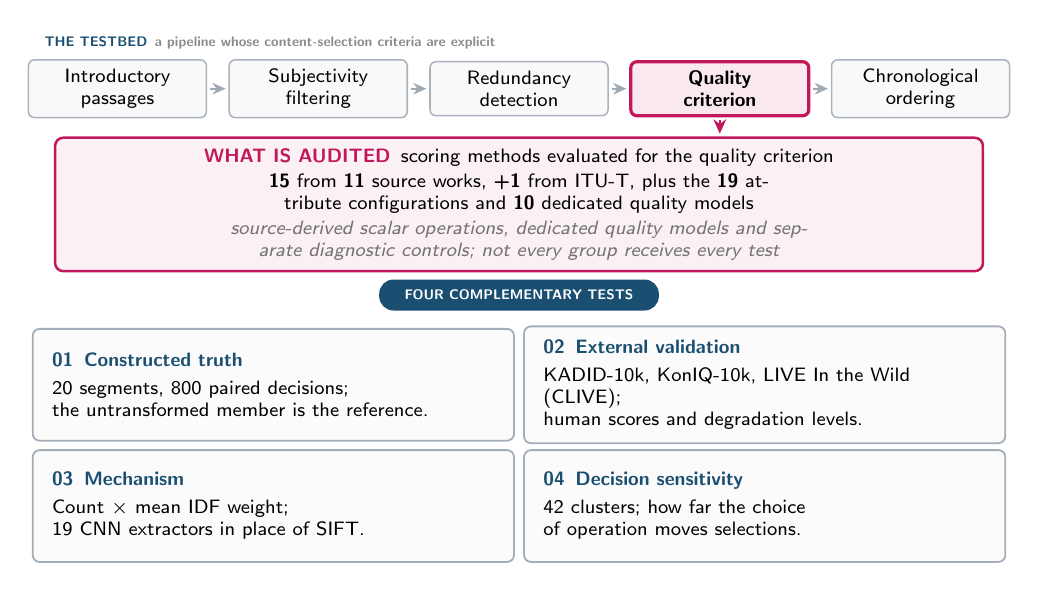
\begin{tikzpicture}[
  stage/.style={rectangle,rounded corners=2.2pt,minimum height=.68cm,
    text width=2.05cm,align=center,font=\sffamily\scriptsize,
    draw=rulegray!85,fill=gray!5,line width=.55pt,inner xsep=3pt},
  focus/.style={stage,draw=focoauditado,fill=focoauditado!10,line width=1.15pt,
    font=\sffamily\bfseries\scriptsize},
  operation/.style={rectangle,rounded corners=3pt,minimum height=.78cm,
    text width=11.55cm,align=center,font=\sffamily\scriptsize,
    draw=focoauditado,fill=focoauditado!6,line width=.9pt,inner ysep=4pt},
  %% ⚠️ altura FIXA nas quatro: a caixa 02 tem tres linhas de corpo e as
  %% outras duas. Como o no cresce em torno do centro, a 02 subia mais que as
  %% vizinhas e encostava na tarja «FOUR COMPLEMENTARY TESTS».
  audit/.style={rectangle,rounded corners=2.5pt,minimum height=1.42cm,
    text width=5.62cm,align=left,font=\sffamily\scriptsize,
    draw=rulegray!90,fill=gray!3,line width=.65pt,inner xsep=7pt,inner ysep=5pt},
  evidencehead/.style={rectangle,rounded corners=5pt,minimum height=.38cm,
    font=\sffamily\bfseries\tiny,text=white,fill=headerblue,draw=headerblue,
    inner xsep=9pt,inner ysep=2.5pt},
  flow/.style={-{Stealth[length=4.8pt,width=4.2pt]},line width=.65pt,
    draw=rulegray!95,shorten <=1pt,shorten >=1pt},
  focusflow/.style={-{Stealth[length=5.2pt,width=4.6pt]},line width=.9pt,
    draw=focoauditado,shorten <=1pt,shorten >=1pt}]

\node[font=\sffamily\bfseries\tiny,text=headerblue,anchor=west]
  at (-6.15,5.50) {THE TESTBED\enspace\textcolor{black!45}{a pipeline whose
  content-selection criteria are explicit}};
\node[stage] (a) at (-5.10,4.92) {Introductory\\passages};
\node[stage] (b) at (-2.55,4.92) {Subjectivity\\filtering};
\node[stage] (c) at (0,4.92) {Redundancy\\detection};
\node[focus] (d) at (2.55,4.92) {Quality\\criterion};
\node[stage] (e) at (5.10,4.92) {Chronological\\ordering};
\draw[flow] (a.east)--(b.west);
\draw[flow] (b.east)--(c.west);
\draw[flow] (c.east)--(d.west);
\draw[flow] (d.east)--(e.west);

\node[operation] (op) at (0,3.45)
  {\textcolor{focoauditado}{\textbf{WHAT IS AUDITED}}\enspace scoring methods evaluated for the
   quality criterion\\[1pt]
   \textbf{15} from \textbf{11} source works, \textbf{+1} from ITU-T, plus the \textbf{19} attribute configurations and \textbf{10} dedicated quality models\\[1pt]
   \textcolor{black!55}{\itshape source-derived scalar operations, dedicated quality models
   and separate diagnostic controls; not every group receives every test}};
\draw[focusflow] (d.south)--(d.south |- op.north);

%% ⛔ 27/09: a tarja ficava em 2,18 e a borda da caixa 01/02 chegava a 1,94:
%% ela sentava EM CIMA da moldura. ⚠️ Nenhuma guarda pega, porque o que se
%% sobrepoe e um traco, nao uma palavra, e `sobrepostos` mede caixas de PALAVRA.
%% ⚠️ 28/09 (cli-3): as caixas tem 5,62 cm + 2x7 pt de margem = ~6,1 cm e estavam a
%% +-2,98 cm: 01/02 e 03/04 se invadiam no meio. Afastadas para +-3,12. A guarda de
%% sobreposicao nao pega, porque mede caixas de PALAVRA e o que encostava era o traco.
\node[evidencehead] (eh) at (0,2.30) {FOUR COMPLEMENTARY TESTS};

\node[audit] (m) at (-3.12,1.16)
  {\textcolor{headerblue}{\textbf{01\enspace Constructed truth}}\\[2pt]
   20 segments, 800 paired decisions;\\the untransformed \mbox{member} is the reference.};
\node[audit] (x) at (3.12,1.16)
  {\textcolor{headerblue}{\textbf{02\enspace External validation}}\\[2pt]
   % ⛔ esta linha quebrava em DUAS no box de 5,25cm e o no crescia para quatro linhas:
   % como o `audit` cresce em torno do centro, ele cobria a tarja acima e o box 04 abaixo.
   % So apareceu ao RENDERIZAR a pagina; o LaTeX nao reclama de no sobreposto.
   KADID-10k, KonIQ-10k, LIVE In the Wild (CLIVE);\\human scores and degradation levels.};
\node[audit] (g) at (-3.12,-.38)
  {\textcolor{headerblue}{\textbf{03\enspace Mechanism}}\\[2pt]
   Count $\times$ mean IDF weight;\\19 CNN extractors in place of SIFT.};
\node[audit] (p) at (3.12,-.38)
  {\textcolor{headerblue}{\textbf{04\enspace Decision sensitivity}}\\[2pt]
   42 clusters; how far the choice\\of operation moves selections.};
\end{tikzpicture}}
\caption{Scope and evidence flow. \textbf{Top}: the content-selection criteria of a
segment-based multi-video summarizer, with the quality criterion as the one under study.
\textbf{Middle}: the scoring methods audited as implementations of that criterion, from the provenance audit. \textbf{Bottom}: the four tests.
Each test reaches a different subset of the audited operations, recorded in Table~S18. All other pipeline stages are held fixed (Section~\ref{sec:data}).}
\label{fig:overview}
\end{figure}

\subsection{Identifying the operations, and reproducing the published rules}\label{sec:prov}

The experimental inventory was selected before the principal scoring runs from operations associated with visual selection in the cited literature. Inclusion required an isolated-frame statistic and a declared direction for that statistic. Graph-based multi-video methods such as MvsGCN~\citep{wu2020mvsgcn} score frames through learned representations and name no quality statistic that can be isolated per frame, so they fall outside this rule. Table~S17 lists the operations that meet it, reimplemented from their sources. The inventory therefore holds three kinds of row: expressions the source specifies, implementations adapted at the input or the normalization, and \emph{combinations aggregated here} from attributes a source names without stating how it combines them. The last kind enters because each attribute it averages satisfies the rule on its own; the aggregation is ours and is marked as such in Table~S22.  The coverage accounting for the archive sweep, the search patterns and the limits of that instrument are recorded in Table~S30.

Table~S16 states the objective and role recorded for each source, and the verbatim excerpt that fixes the validation evidence is in Tables~S24 and~S25. Standalone ordering is distinguished from classifier features, terms within a larger objective and threshold-based filtering. Validation evidence is coded by its object, attribute, module or summary, and reference, such as human ratings, summary evaluation or ablation. All \fontesTrabalhos{} source works were read in full.

Implementations reproduce the specified expression where its inputs are available; task and interface adaptations are recorded separately in Table~S22. In particular, saliency area uses a spectral-residual map ~\citep{hou2007spectral} rather than the source's learned map; the rule of Ref.~\citep{korolkov2025keyframe} uses normalization over the benchmark candidates, including original and transformed members; and the comparator of Ref.~\citep{ke2006highlevel} is a Gaussian naive Bayes classifier trained on constructed-degradation labels with leave-one-segment-out validation. These variants evaluate adapted components.

Polarity is attached to the actual quantity extracted. In Ref.~\citep{jeong2016static}, raw pixel variance is transformed into a badness penalty before entering a minimized cost. The present statistic is the grey-level dispersion, implemented as the standard deviation rather than the variance the source states. That source names three badness terms, contrast, blur and skew, inside one multiplicative cost, and only the contrast term is audited here: the other two are not separable from the published expression as isolated-frame statistics, which is the same inclusion rule that admits the contrast term. A second polarity ambiguity appears in Ref.~\citep{xu2024property}, which states that all five entity scores are normalized to $[0,1]$ with higher meaning better while using BRISQUE, whose published direction is lower-is-better, without stating an inversion; the direction evaluated here is the one the scorer itself declares. 

\subsection{Data and units of analysis}\label{sec:data}

KADID-10k contains 10,125 distorted images generated from 81 references, 25 distortion types and five levels ~\citep{lin2019kadid}. Its released opinion-score field is named `dmos` but increases with quality. KonIQ-10k and LIVE In the Wild, also denoted CLIVE, supply authentic distortions and Mean Opinion Scores (MOS) ~\citep{ghadiyaram2016clive,hosu2020koniq}. No dedicated NR-IQA model is retrained or fine-tuned. The fitted combination variants are identified separately.

HSMVideoSumm provides the modular broadcast-news testbed ~\citep{barbieri2021tese,barbieri2021content,moraes2024hsmvideosumm}. Its visual-word operation is one of the audited works of this study: the source proposes scoring a segment by the sum of TF-IDF weights over a $K=300$ visual-word vocabulary~\citep{barbieri2021tese}, and the released code is the implementation these measurements run~\citep{moraes2024hsmvideosumm}. \textbf{It was chosen because it is modular, open and documented at the stage this audit targets}: the quality criterion is a replaceable component, so an operation can be swapped without touching the rest of the pipeline, which is what the substitution analyses require. It was also developed in our laboratory, which gave access to the released code and to the corpus it runs on. That source defines the criterion of the stage audited here as whether a segment \emph{contains images of interest}, a relevance criterion, and the same study reports that aesthetic quality was not relevant to its participants. We reuse its modular pipeline to evaluate a separate requirement, technical fidelity, defined in this audit. Original redundancy groups and the remaining pipeline stages are retained.

The application uses the \disClusters{} multi-member clusters produced by the redundancy stage over 19 of the 21 topics, containing 93 segment slots and 83 distinct segments. Some segments occupy more than one cluster. Still-image scorers ordinarily receive frames sampled at one frame per second and use the segment mean
\begin{equation}
S(s)=\frac{1}{n_s}\sum_{i=1}^{n_s}\phi(f_i),
\label{eq:meanpool}
\end{equation}
where $\phi(f_i)$ is the frame score. The SIFT+BoVW counting operation instead uses its own keyframe selector and a vocabulary of $K=300$ visual words.

Each implementation ranks candidates within a fixed cluster and selects the highest-ranked candidate after polarity alignment. The two treatments are reported separately and distinguish the effects of implementation and scoring. The complete-implementation comparison preserves each operation's own sampling and aggregation. The matched-input control supplies both scorers with the same, at most ten, uniformly spaced frames and mean pooling. Only the matched-input control isolates scoring under a common input regime.

The independent unit follows the analysis: KADID reference image for synthetic-distortion sensitivity; source-aware topic block for the primary constructed-pair inference; and news topic for application inference. Segment-block and hierarchical alternatives quantify sensitivity to dependence assumptions. Individual frames, transformations and overlapping segment slots are not treated as independent replicates.

\subsection{Scorers, references and polarity}\label{sec:methods}

The complete-case comparator set contains \invModelos{} no-reference image quality assessment (NR-IQA) models: BRISQUE, NIQE, DBCNN, HyperIQA, MUSIQ, TOPIQ, CLIP-IQA, CLIP-IQA$+$, LIQE and QualiCLIP. ARNIQA and TReS extend completed axes but do not enter complete-case screening ~\citep{agnolucci2024arniqa,golestaneh2022tres}; MANIQA was incomplete at the scoring freeze ~\citep{yang2022maniqa}. Released checkpoint, supervision, preprocessing and decision polarity identify the evaluated configuration in Table~\ref{tab:methods}.

%% ⭐ 28/09 (parecer): a coluna das bases nao vistas repetia a mesma string em 12 linhas e e derivavel
%% do treino; «Role» era C em 12 de 13. A regra das nao vistas vai UMA vez na legenda, e as
%% faixas separam candidato, referencia e cobertura parcial, que antes dividiam um bloco.
\begin{table}[!tbp]
\centering
\caption{No-reference comparators and reference. \emph{Opinion training}: the database
whose human scores trained the released checkpoint; \emph{none} marks opinion-unaware
models. The transfer condition is tested on every evaluated database (KADID-10k,
KonIQ-10k, LIVE In the Wild) absent from that training; the LIVE database of the BRISQUE
checkpoint is not among them, so all three are unseen for it. \emph{Pol.}: declared polarity,
fixed before evaluation; \polup{}, a higher score means better quality; \poldown{}, a lower
score means better quality. Constructs, released weights, endpoints and preprocessing, with the diagnostic
controls and the 19-extractor ablation, are in Table~S12.}
\label{tab:methods}
\small
\renewcommand{\arraystretch}{1.1}
\begin{tabular}{@{}p{3.4cm}p{6.2cm}c@{}}
\toprule
\rowcolor{headerblue}
\hd{Method} & \hd{Opinion training} & \hd{Pol.} \\
\midrule
\multicolumn{3}{@{}l}{\emph{Candidates, opinion-unaware}}\\[1pt]
NIQE & none & \poldown \\
\rowcolor{rowlight}CLIP-IQA & none & \polup \\
QualiCLIP & none & \polup \\
\addlinespace[3pt]
\multicolumn{3}{@{}l}{\emph{Candidates, opinion-trained}}\\[1pt]
BRISQUE & LIVE~\citep{sheikh2006live} & \poldown \\
\rowcolor{rowlight}DBCNN & KonIQ-10k & \polup \\
HyperIQA & KonIQ-10k & \polup \\
\rowcolor{rowlight}MUSIQ & KonIQ-10k & \polup \\
TOPIQ & KonIQ-10k & \polup \\
\rowcolor{rowlight}CLIP-IQA$+$ & KonIQ-10k & \polup \\
LIQE & KonIQ-10k & \polup \\
\addlinespace[3pt]
\multicolumn{3}{@{}l}{\emph{Reference}}\\[1pt]
Q-Align & multiple databases & \polup \\
\addlinespace[3pt]
\multicolumn{3}{@{}l}{\emph{Partial coverage, outside screening}}\\[1pt]
ARNIQA & KonIQ-10k & \polup \\
\rowcolor{rowlight}TReS & KonIQ-10k & \polup \\
\bottomrule
\end{tabular}
\end{table}

Diagnostic controls include keypoint density, spatial information, a second inverse-document-frequency formulation and deep-feature measurements. The deep controls use DINOv2 ~\citep{oquab2024dinov2}, specifically ViT-S/14 with registers ~\citep{darcet2024registers} at half precision (FP16), averaging patch tokens into a 384-dimensional frame vector. They measure vector norm, the negated mean distance of frames to their segment centroid, and distance to the centroid of the operational cluster, which Ref.~\citep{jeong2016static} adds to its quality terms as the distance of a frame from its cluster centre; here it is computed between segment vectors. On the constructed pairs the degraded copy joins the original's cluster and the centroid of all members decides between the two. A separate ablation over 19 convolutional extractors replaces SIFT while preserving vocabulary construction, weighting and aggregation. Two counting-descriptor substitutions were also excluded. SURF is excluded for lack of a redistributable implementation, being patented and absent from the OpenCV build these measurements ran on. The second was excluded because exchanging it would require recalibrating the key-frame selector that runs before the score. Table~S12 records configurations, endpoints and the build environment.

Q-Align, an architecturally distinct model at the inventory freeze, is the in-domain reference for the NR-IQA candidate set; LIQE is the reference for the literature-derived operations. The two groups are compared directly only in a common-reference analysis (Section~\ref{sec:screen_results}).

DOVER~\citep{wu2023dover} scores the selected outputs as model-based evidence of output quality, independently of eligibility; its protocol and results are in the supplement.

For a score $q$ and target $y$, direction-aligned Spearman correlation is $\rho^*=s_m s_y\rho(q,y)$, where $s_m=+1$ for a higher-is-better score and $-1$ otherwise; $s_y$ specifies the target's direction. All released opinion targets used here have $s_y=+1$. In contrast, larger distortion levels $d$ denote more degradation, so sensitivity requires $s_y=-1$ and $\rho^*_{\mathrm{level}}=-s_m\rho(q,d)$. This target-specific definition separates a polarity convention from a genuine reversal.

For the \resCombinacoes{} attribute configurations, an additional oracle-polarity diagnostic uses the absolute correlation separately on each database or axis. It gives a favourable retrospective orientation, since the sign is inferred from the test outcomes; conclusions about transfer rely on the declared directions.

\subsection{Controlled degradation and constructed truth}\label{sec:controlled}

A seeded draw without replacement selects twenty of the 83 broadcast segments, which come from \invRotulos{} of the 19 operational topics (Table~S2); two of those labels share source videos and overlapping segments, so they are merged into \invBlocosN{} source-aware blocks. Eight deterministic transformations at five levels produce $20\times8\times5=800$ original--transformed comparisons per fully covered operation. The transformations are darkening, motion blur, Gaussian blur, H.264 recompression, downscale-and-restore, desaturation, white noise and JPEG compression.

The untransformed member is the fidelity reference the protocol defines. A sensitivity analysis excludes darkening and desaturation, which need not worsen appearance for every viewer. With $W$, $L$ and $T$ the pairs in which an operation prefers the untransformed member, the transformed one or neither, \emph{strict} accuracy is $W/(W+L+T)$ and \emph{decisive} accuracy $W/(W+L)$; the two are not interchangeable, so the main tables report strict accuracy, the per-cell tests decisive accuracy, and a descriptive inversion is $L>W$. Only \empOps{} of the \fontesDaLiteratura{} operations tie at all.

For each operation--transformation cell, exact sign-flip randomization uses source-aware block means and enumerates all $2^b$ sign assignments. The reported directional tests use the lower tail with Holm correction over \fontesDaLiteratura{} operations and eight transformations, or \invTestes{} tests. The convention matters at this sample size: with \invBlocosN{} blocks the smallest attainable one-sided $p$ is $\invPmin{}$ against a first Holm threshold of $\invCorteHolm{}$, so a two-sided convention would reject nothing. Segment-level results provide an alternative dependence assumption. Table~S27 reports cell-level tests and Table~S26 the alternative intervals.

A second analysis correlates score with transformation level within each segment--type combination. On KADID, correlation across five levels is computed separately for each reference image and distortion type before averaging. This prevents the many derivatives of one reference from inflating the number of independent source images. 

\subsection{Screening and application inference}\label{sec:screen}

Scoring methods are evaluated against three eligibility conditions, which admit methods without ordering them. The sensitivity condition uses KADID only. It requires mean direction-aligned Spearman Rank Correlation Coefficient (SRCC) of at least .50, with at least 15 of the 25 distortion types exceeding .50 after reference-wise averaging. The eight-type broadcast experiment is complementary and does not determine this condition. The external-transfer condition requires database-wide direction-aligned SRCC of at least .65 on every database absent from a checkpoint's opinion training. Threshold sensitivity is reported in Table~S9.

The two aggregations of attribute configurations are author-defined. The $z$-score mean re-estimates a mean and a standard deviation per operation on each database, so its KonIQ-10k figure uses a normalization fitted on KonIQ-10k. The ridge is fitted on KADID-10k with the distortion level as target and a fixed penalty of one over standardized inputs, so its KADID figures are in-sample and its KonIQ-10k figure applies the KADID coefficients. Both are reported as diagnostic associations, and the in-sample ridge is an optimistic diagnostic that only shows whether a negative outcome survives the more favourable aggregation.

The in-domain condition requires above-chance agreement with the designated reference and a positive lower bound of its 95\% topic-block bootstrap confidence interval. For cluster $c$ with $k_c$ candidates, independent uniform choices agree with probability $1/k_c$. Across the common \disClusters{} clusters, $\bar p_e=|C|^{-1}\sum_{c\in C}1/k_c=\dupPisoDec{}$, and normalized agreement is $\kappa_{\mathrm{uniform}}=(p_o-\bar p_e)/(1-\bar p_e)$. This is a uniform-choice correction, not Cohen's kappa.

 

The principal inventory, scoring runs and caches were frozen on 23 August 2026; dependence-aware derived analyses were subsequently computed from those caches, and the deep-proxy controls were completed on 21 September, with the cluster-centre test on the constructed pairs registered and run on 27 September. Archived prediction statements refer only to their specified diagnostic tests.

\paragraph{Use of large language models.} Language-model assistants were used to write
the analysis and verification scripts and to draft and revise the text. Every quantitative
statement reaches the manuscript through a macro emitted by a versioned script from a
stored result file, and is checked by the consistency suite released with the package; the
authors took every methodological decision and are responsible for the content. The full
declaration, naming the assistants, is in the Statements and Declarations.

\section{Results}\label{sec:results}

%% ⛔ 21/09 (parecer, E00, criterios 21, 26, 29, 45, 48): o roteiro dizia «six blocks»,
%% apontava para a Secao 3.1, que e METODOLOGIA, e punha o mecanismo por ultimo quando
%% ele e o terceiro. Sao sete subsecoes; a ordem abaixo e a ordem em que aparecem.
%% ⛔ 22/09 (parecer v2, V2-042): o roteiro de sete blocos repetia o que os titulos das
%% subsecoes ja dizem. ⛔ 25/09 (parecer v11): a frase de transicao que ficou no lugar dele
%% fazia o mesmo trabalho duas vezes, e saiu. Os titulos carregam a ordem sozinhos.

\subsection{Classes of scoring method, and what the testbed instantiates}\label{sec:taxonomy_results}

%% ⛔ 22/09 (parecer v2, V2-045): «confirmed corpus», «account for the remainder» e «the
%% three screened here» implicavam particao e cobertura que a propria tabela nega (os
%% grupos se sobrepoem, ha trabalhos sem nenhum, e a classe contextual nao recebe o mesmo
%% teste). A frase passa a falar dos conjuntos efetivamente avaliados.
Table~\ref{tab:taxonomy} gives what the testbed instantiates in each class, and the
screening of Section~\ref{sec:screen_results} covers the scalar operations that the
isolated-image protocol admits. Of the three deep proxies implemented over the DINOv2
ViT-S/14 embedding, only the norm of the feature vector is an absolute per-frame score.
Frame coherence needs several frames and the distance to the cluster centre, the quality
term of Ref.~\citep{jeong2016static}, needs a candidate set, so both are \emph{not
applicable} to the external databases, which score isolated images. The feature-norm reading
is a construction of ours used as a diagnostic: no audited source states it. All three appear
in the last band of Table~\ref{tab:constructed}.

The class does not fail as a block. The norm averages \taxNormaPar{} per cent and ranks
the degraded copy above the original on \taxNormaInverte{} of the eight types: degrading
a frame lengthens its representation, so reading vector length as quality is reversed. It fails outside the pairs as well: its lowest correlation on an unseen database is \taxNormaExt{}, and its agreement with the reference on the operational clusters \taxNormaPiso{}.
Frame coherence averages \taxCoerPar{} per cent and inverts on \taxCoerInverte{} type. Its
score is the negated mean distance of the frames to their own centroid, so a per-frame
perturbation that scatters the representations, white noise among them, lowers it. Both
readings were registered as opposing predictions before the measuring script was run. On
the pipeline's own clusters frame coherence agrees with the reference at
\taxCoerKappa{}, a point estimate without the interval the in-domain condition requires.

Two candidates are equidistant from their own midpoint, so the cluster-centre distance
cannot decide a pair alone. Placed in the original's operational cluster, with the
centroid computed over all members, it prefers the original on \taxCentPar{} per cent of
the 800 pairs (95\% CI \taxCentIC{} by segment) and on no type falls below
\taxCentMin{}, under every dedicated model of Table~\ref{tab:constructed}, the lowest of which reaches \taxModeloMin{}. Most of that preference does not need the cluster: in a control added after this
result, members drawn from other topics leave \taxCentOutros{} per cent, and the real
cluster adds \taxCentDif{} points, computed pair by pair (\taxCentDifIC{}). The proxy mostly registers
that a degraded copy moves away from typical broadcast content in the embedding. On the operational clusters it decides only in the \taxCentroideDecide{} with three or more members, too few for the in-domain condition.

\subsection{Responses to controlled degradation}\label{sec:class}

All \fontesDaLiteratura{} operations prefer the degraded copy on at least one type;
\resRuido{} do so under white noise, and \resZeroRuido{} are wrong on all 100 noise pairs
(Figure~S3).

Under the one-sided, Holm-corrected randomization of Section~\ref{sec:controlled}, how many inversions survive depends on the nested unit. Over the 20 segments, \invSig{} of the \invCelulas{}
cells below chance survive, in \invOpsSig{} of the \fontesDaLiteratura{} operations;
over topics, the more conservative reading, \invSigTop{} cells in \invOpsSigTop{}
operations. The topic unit is \invBlocos{} source-aware blocks; keeping the two shared
labels apart would leave \invSigRotulo{} cells. What does not depend on the unit is the core: the
\invPerfeitas{} cells in which an operation is wrong on all one hundred pairs survive in every unit. The same test leaves
\invModelosLimpos{} of the \invModelos{} published models with no type below chance, and
removing the two types aligned with an operation's own attribute leaves all
\tipoSemAlinhados{} still inverting. Table~S27 lists the \invCelulas{} cells with the
verdict under each unit, and Table~S26 recomputes every interval under the rival unit.

White noise concentrates the failures, and it is the only tested transformation
whose median energy ratio exceeds one. Measured as the median ratio of Laplacian
variance after to before, \eneAdicionam{} of the eight types raises it: noise multiplies
it by \eneRuido{},
every other type leaves it at or below \eneMaiorSemRuido{} of the original, JPEG included at \eneJpeg{}; Figure~S2 shows the paired accuracy of the fifteen operations against the same eight types. Laplacian variance indicates local high-frequency content; these operations are statistics of local
structure, and additive noise raises such statistics, so an operation reading more
structure as more quality prefers the noisier frame. Across the fifteen that is a pattern, and Section~\ref{sec:mechanism} measures the chain end to end for the SIFT+BoVW score.

The same 800 pairs place the evaluated scalar scorers, the no-reference models and the three deep proxies on one scale (Table~\ref{tab:constructed}). SIFT+BoVW is not an outlier among the scorers this
literature supplies: it is correct on \mchImplantada{}\%
of the pairs, which sits at the median of the literature-derived operations
(\tipMediana{}\%; Table~S32). LIQE is correct on \mchLiqe{}\%, a paired difference of
$+\mchDif{}$ points, with 95\% CI $\mchICTop{}$ over the \mchTopicos{} source-aware blocks, $\mchICSeg{}$ by segment block and $\mchICTopSem{}$ under the separate-label grouping. Table~S32 records the literature operations with their
accuracies and the comparisons behind each.

\begin{table}[!ht]
\centering
\caption{\textbf{Strict} accuracy $W/(W+L+T)$, in per cent, on 800 unmodified--degraded broadcast pairs: 20
segments, eight types and five levels. \emph{dark}: darkening; \emph{motion}: motion
blur; \emph{blur}: Gaussian blur; \emph{H.264}: video recompression; \emph{rescale}:
downscale and restore; \emph{satur.}: desaturation; \emph{noise}: white noise. Values below the 50\% chance
floor are \textbf{descriptive inversions} where $L>W$, in bold and in colour;
which of them survive the corrected exact tests is reported in the text and in Table~S27.
No row ties, so strict and decisive accuracy coincide, except the cluster-centre distance, whose \taxCentMeios{} pairs with the original in two disagreeing clusters count one half. The first band holds SIFT+BoVW and the three best-scoring literature operations. ARNIQA appears on this paired axis but stays outside the
complete-case screening of Section~\ref{sec:screen_results}. The last band holds the deep proxies of Section~\ref{sec:taxonomy_results}; for the cluster-centre distance the degraded copy joins the original's cluster.}
\label{tab:constructed}
\scriptsize
\setlength{\tabcolsep}{1.9pt}
\begin{tabular}{@{}lccccccccc@{}}
\toprule
\textbf{Method} & \textbf{dark} & \textbf{motion} & \textbf{blur} & \textbf{H.264}
& \textbf{rescale} & \textbf{satur.} & \textbf{noise} & \textbf{JPEG} & \textbf{mean} \\
\midrule
SIFT+BoVW & 100 & 100 & 90 & 90 & 88 &
\textcolor{accentred}{\textbf{39}} & \textcolor{accentred}{\textbf{8}} &
\textcolor{accentred}{\textbf{6}} & \textbf{65.1} \\
Mean rule~\citep{srinivas2016rank} & 100 & 100 & 100 & 100 & 100 & 98 & \textcolor{accentred}{\textbf{29}} & 69 & \textbf{87.0} \\
Colourfulness~\citep{hasler2003colorfulness} & 100 & 100 & 100 & 100 & 100 & 100 & \textcolor{accentred}{\textbf{3}} & 79 & \textbf{85.2} \\
Averaged aesthetics~\citep{gygli2014summe} & 100 & 100 & 100 & 100 & 100 & 100 & \textcolor{accentred}{\textbf{3}} & 67 & \textbf{83.8} \\
\midrule
LIQE & 97 & 100 & 100 & 100 & 100 & 100 & 99 & 100 & \textbf{99.5} \\
TOPIQ & 93 & 100 & 100 & 100 & 100 & 93 & 100 & 100 & 98.2 \\
MUSIQ & 93 & 100 & 100 & 100 & 100 & 86 & 100 & 100 & 97.4 \\
QualiCLIP & 99 & 100 & 95 & 100 & 96 & 76 & 96 & 71 & 91.6 \\
ARNIQA & 91 & 100 & 99 & 98 & 100 & 61 & 82 & 98 & 91.1 \\
DBCNN & 84 & 97 & 92 & 97 & 95 & 92 & 85 & 81 & 90.4 \\
NIQE & 100 & 100 & 98 & 97 & 98 & \textcolor{accentred}{\textbf{0}} & 100 & 96 & 86.1 \\
CLIP-IQA$+$ & 76 & 99 & 79 & 100 & 91 & 87 & 84 & 64 & 85.0 \\
HyperIQA & \textcolor{accentred}{\textbf{47}} & 100 & 100 & 100 & 100 & \textcolor{accentred}{\textbf{30}} & 100 & 100 & 84.6 \\
CLIP-IQA & 58 & 100 & 83 & 100 & 92 & 91 & 55 & 76 & 81.9 \\
BRISQUE & 100 & 100 & 100 & 99 & 100 & \textcolor{accentred}{\textbf{0}} & 67 & 80 & 80.8 \\
\midrule
Feature-vector norm & \textcolor{accentred}{\textbf{33}} & \textcolor{accentred}{\textbf{10}} & \textcolor{accentred}{\textbf{19}} & \textcolor{accentred}{\textbf{10}} & \textcolor{accentred}{\textbf{19}} & 60 & \textcolor{accentred}{\textbf{14}} & \textcolor{accentred}{\textbf{14}} & \textcolor{accentred}{\textbf{22.4}} \\
Frame coherence & 62 & 50 & 76 & \textcolor{accentred}{\textbf{44}} & 77 & 63 & 72 & 86 & 66.2 \\
Cluster-centre distance & 56 & 86 & 65 & 77 & 71 & 76 & 91 & 72 & 74.1 \\
\bottomrule
\end{tabular}
\end{table}

Excluding darkening and desaturation leaves 600
comparisons and does not repair the SIFT+BoVW operation: its accuracy is 63.7\%,
whereas LIQE reaches 99.8\% and Q-Align 100\% (Table~S11). 

The average conceals the diagnostic result: SIFT+BoVW is at or above 88\% on five
types but selects the degraded copy in 92\% of white-noise pairs and 94\% of JPEG pairs.
Section~\ref{sec:mechanism} examines what the descriptor count and the
inverse-document-frequency weighting contribute to those reversals.

Q-Align is correct on 98.2\% of these pairs (95\% CI $[97.2,99.1]$), which
supports its technical-degradation competence on this broadcast content. The exact downstream DOVER technical branch (DOVER-T) output
reaches 97.6\% ($[96.1,99.0]$), or 99.8\% ($[99.5,100]$) without darkening and
desaturation. The registered prediction audit, including the two overlay predictions, is in Table~S11.
\subsection{Why a count of local detail reads as quality}\label{sec:mechanism}

The decomposition below separates the contribution of the descriptor count from that of
the mean rarity weight. 

\begin{equation}
\mathrm{score}_i=\sum_v\mathrm{tf}_{iv}\mathrm{idf}_v
=D_i\underbrace{\sum_v p_i(v)\mathrm{idf}_v}_{\overline{\mathrm{idf}}_i}.
\label{eq:factor}
\end{equation}
Here $D_i$ is the number of descriptors the extractor finds in segment $i$,
$\mathrm{tf}_{iv}$ how many fall in visual word $v$, and $p_i(v)$ that count as a fraction
of $D_i$, so the score is a descriptor count times a mean inverse-document weight,
and which channel dominates is measured rather than assumed. %% ⛔ 22/09 (parecer v2): «a different weighting breaks it» e falso. Trocar um vetor de
%% pesos constantes por outro preserva a identidade; o que a quebra e o peso deixar de ser
%% constante por palavra, ou a agregacao deixar de ser soma sobre frequencias cruas.
%% ⛔ 25/09 (parecer v10, 2.1): e «uma agregacao que nao e essa soma REMOVE o fator de
%% contagem» tambem era falso, no outro sentido. A media sobre F quadros da
%% (D_i/F)*idf_barra: o fator de contagem SOBREVIVE, virando contagem POR QUADRO. So a
%% divisao pela contagem o remove. A frase agora diz cada caso pela sua definicao.
The identity is algebraic and holds for any weights, since $p_i(v)=\mathrm{tf}_{iv}/D_i$
by definition, whenever the aggregation is a sum over raw term frequencies and $D_i>0$.
Averaging frame scores leaves a count-per-frame factor, $(D_i/F)\,\overline{\mathrm{idf}}_i$
over $F$ frames, and only dividing by the descriptor count removes it.

In the deployment regime the count channel dominates: $\rho(S_{\mathrm{dep}},D)
=\mecRhoContagem{}$, and on the 800 constructed pairs the signs of the score and count differences
agree in \mecConcordam{}, the three exceptions differing by at most \excDelta{}
descriptors against a median count of \excMediana{}. \textbf{Replacing the score by that count leaves every representative choice unchanged}, \redEscolhas{} of \redDe{} on the application clusters, while replacing it by the number of key frames the selector retains preserves only \redQuadros{}; Table~S33 reports the reduction. The degraded copy carries more
descriptors in 92\% of noise pairs and 95\% of JPEG pairs, so noise and blocking
raise the count channel of Eq.~\ref{eq:factor} while structure-removing distortions
happen to move it in the direction of fidelity: the score is responsive, but not
consistently to quality. The 19 convolutional extractors average 44.9\% (CI $[41.0,48.9]$)
and remain dominated by their descriptor count, which refutes the registered
prediction that fixed feature maps would force chance performance.

Exchanging the extractor therefore changes individual choices without making the ordering
a better predictor of quality, and the normalization variants evaluated here did
not repair the reading either. Figure~S1 shows the two channels; the supplement gives the exact relation between the two inverse-document-frequency formulations, which differ by an additive count term, and the per-extractor external correlations.

\subsection{Literature-derived composites and source-specified rules}\label{sec:combinations}

\textbf{Nineteen attribute configurations combine the implemented statistics} (Table~S29). Twelve
combine more than one term and seven are single terms, aggregated by a $z$-score mean or a ridge model defined here. None of the nineteen satisfies both external screening
requirements under either aggregation. One $z$-score combination passes sensitivity with
a within-reference mean of $.524$ on 17 of 25 types, above the requirement no
individual operation met, but its KonIQ-10k correlation is $\rho^{*}=.061$ against a
requirement of $.65$.

Several sources specify how their own terms combine, and those specifications were
implemented over the same attribute vector so the comparison isolates the rule.
%% ⛔ 22/09 (parecer v2, V2-062): a reescrita apagou POR QUE estes numeros diferem dos da
%% Tabela 6, e o leitor ficava com 74,3 contra 77,5 sem explicacao. Nao e inconsistencia:
%% o contraste exclui o tipo alinhado a construcao do modulo. Populacao e exclusao saem
%% por macro para nao sumirem de novo num corte.
In both sources that specify a complete module, the published rule scores below
its own best component, and each contrast excludes the degradation type aligned
with that module's own construction, so it runs on seven types rather than eight. For Ref.~\citep{qaroush2025diversity} the contrast excludes \vaTipoFora{} and uses \vaPares{}
comparisons from 20 segments: \vaModulo{} per cent against \vaMelhorMembro{} for its best
term, colourfulness, a paired contrast of \vaContraste{} points with an interval of \vaIC{} that excludes
zero. For Ref.~\citep{korolkov2025keyframe} it excludes \koTipoFora{} and uses \koPares{}
comparisons from the \koN{} of \koDe{} segments carrying both inputs: \koModulo{} against
\koMelhorMembro{}, a contrast of \koContraste{} points with a segment-block interval of
\koIC{} that touches zero. The source-level synthesis of Section~\ref{sec:synthesis} reports the corresponding
all-eight-type means instead, \vaMediaOito{} and \koMediaOito{} per cent, which is why the
two sets of numbers differ. The comparator is each module's best component, chosen after the results were seen. The adapted classifier of Ref.~\citep{ke2006highlevel} reaches \regraKe{} per cent against \regraMedia{}
for the unweighted mean, as a task adaptation (Section~\ref{sec:prov}).

In two sources the published expression carries the opposite sign to the property
the surrounding text names for it: the contrast term of the objective of Ref.~\citep{qaroush2025diversity} is the difference between the standard deviations before and after histogram equalization, not a measure of contrast itself, and in a controlled sweep over \ctNiveis{} levels it is perfectly inversely associated, at $\ctRho{}$, with the contrast used to build the inputs. The result is established for the tested sweep. The
brightness term of the module of Ref.~\citep{korolkov2025keyframe} needs no such condition: it is described as
penalizing over-exposure while the mean luminance it specifies is monotone in exposure and
enters with a positive weight. Both statements concern the formulations as published; Table~S21 gives the sweep.

\subsection{External validation and screening}\label{sec:screen_results}

No evaluated operation clears either external eligibility condition. The best
within-reference mean among the fifteen is $.298$ against a requirement of $.50$, and the
best lowest-unseen correlation is $.139$ against $.65$; spatial information carries no verdict, reaching $.218$ only in an increasing direction its source does not declare. \textbf{Which database decides the failure is not fixed}: for \basePiorKadid{} of the \fontesDaLiteratura{} operations the worst case is on the synthetic KADID-10k and for the remaining \basePiorKoniq{} it is on the authentic KonIQ-10k, so the generalization axis is not carried by a single database. Table~\ref{tab:families} reports each
group's best value per axis. The result is stable: across \refB{} resamples of the reference images, \refViram{} of the fifteen changes verdict, and four operations are \emph{negative} on the first requirement, their response running against the direction their own use assumes. \textbf{The fifteen screened literature operations all belong to the first class}, and SIFT+BoVW is the one screened member of the second: the isolated-image protocol admits scalar per-frame statistics, and that is what the summarization literature supplies. Table~\ref{tab:taxonomy} shows the other side of the same asymmetry, that the class of dedicated models, with ten operations instantiated here, is matched to one paper in the archive. The narrow coverage of this screening therefore follows from what the field publishes.

\begin{table}[!ht]
\centering
\caption{\textbf{External screening by method class} (Table~\ref{tab:taxonomy}). Each cell is the maximum over its class on that axis alone, so \textbf{the two maxima need not belong to the same member}. \emph{Clears both external} counts the members passing sensitivity and generalization together; \textbf{the in-domain floor is a third condition, reported separately}. Spatial information declares no direction and carries no verdict; the heuristics row counts 16 computed and 15 evaluated, and the bag-of-visual-words row 3 computed and 1 evaluated: the other two, keypoint density and the 19-extractor ablation, are diagnostics rather than published scores. Deep proxies read context and fall outside the isolated-image protocol (Section~\ref{sec:taxonomy_results}). The two source-specified rules are not screened (Section~\ref{sec:combinations}). $^{\star}$Diagnostic, not a published class: generalization is the KonIQ-10k association under a data-derived orientation with normalization re-estimated per database, which makes its zero conservative. Per-operation values are in the supplement.}
\label{tab:families}
\small
\setlength{\tabcolsep}{7pt}
\renewcommand{\arraystretch}{1.0}
\begin{tabular}{@{}>{\raggedright\arraybackslash}p{3.5cm} c r r c@{}}
\toprule
\rowcolor{headerblue}
\hd{Evaluated group} & \hd{$n$} & \hd{Best sens.} & \hd{Best gen.} & \hd{Clears both external} \\
\midrule
\rowcolor{focoauditado!12}Low-level pixel heuristics & 16 & $+.298$ & $+.139$ & 0 of 15 evaluated \\
\rowcolor{focoauditado!12}Visual-word counting: SIFT+BoVW \citep{barbieri2021tese} & 3 & $-.077$ & $-.445$ & 0 of 1 evaluated \\
\rowcolor{accentgreen!14}Dedicated NR-IQA models & 10 & $+.849$ & $+.723$ & \textbf{3 of 10} \\
\rowcolor{focoauditado!7}Deep representativeness proxies & 3 & --- & --- & \textcolor{black!45}{not screened} (Section~\ref{sec:taxonomy_results}) \\
\midrule
\rowcolor{rowlight}\emph{Attribute configurations (diagnostic)}$^{\star}$ & 19 & $+.524$ & $+.601$ & 0 of 19 \ \tiny(1 clears sens.) \\
\midrule
\bottomrule
\end{tabular}
\end{table}


%% ⭐ 28/09 (parecer + decisao do Jader): o detalhe de elegibilidade POR MODELO, o piso por
%% modelo, a comparacao de referencia comum e o custo sao benchmark de modelo, nao auditoria
%% das operacoes, e foram para o suplementar (secao «Model eligibility and output quality»).
%% Aqui fica o que responde a pergunta do artigo.
Three dedicated models are eligible, LIQE, QualiCLIP and CLIP-IQA$+$, and the set is stable
under the threshold variations of Table~S9. Within-reference KADID sensitivity separates the
SIFT+BoVW operation sharply: its mean is $-.077$ (95\% CI $[-.124,-.030]$) with 5 of 25
types above .50, against .807 to .849 for the three eligible methods. On the in-domain
floor, against LIQE, the reference the protocol assigns to the literature-derived
operations, it agrees on \subResta{} of \pisoDe{} clusters
($\kappa_{\mathrm{uniform}}=\subKappa{}$), an interval that crosses chance. Several
literature-derived operations meet this condition on unmodified broadcasts despite failing
both external ones, and \pisoFrageis{} lose that pass when one topic is removed. The sensitivity verdict is also conditional on the benchmark: applied to the constructed pairs, the same rule admits six of the fifteen, and none meets it on both. The
per-model floor intervals, the common-reference comparison, the regime term behind the
KADID gap and the cost are in the supplement.

\FloatBarrier

\subsection{Effect of the implementation on content selection}\label{sec:menu}

Across the 42 operational clusters, \disOps{} evaluated scoring implementations
of the one criterion produce \disResumos{} distinct representative selections, with the
decoded frames and the remaining criteria held fixed, and at least two disagree in
\disClusters{} of the 42. Every candidate in every cluster is selected by at least one
operation, so the mean of $\escMedia{}$ distinct choices per cluster is the ceiling the
cluster sizes allow, and the outputs that match do so because the operations compute the
same quantity. Implementation identity therefore changes the selection under a
fixed candidate set. This measures selection sensitivity and uses no reference method; it does not identify the better representative.

Pairwise, the median agreement is \dupComMediana{} per cent against a chance floor of
$\dupPiso{}$, and \dupComAbaixo{} of the \dupComPares{} pairs agree below chance
(Figure~\ref{fig:menu}). Collapsing the duplicate computations leaves \dupDistintas{}
distinct operations and \dupPares{} pairs, with a median of \dupMediana{}, so the
spread is not an artefact of counting one computation twice. Among the source
works read in full, none evaluates its operation against the others on common material.

\begin{figure}[!ht]
\centering
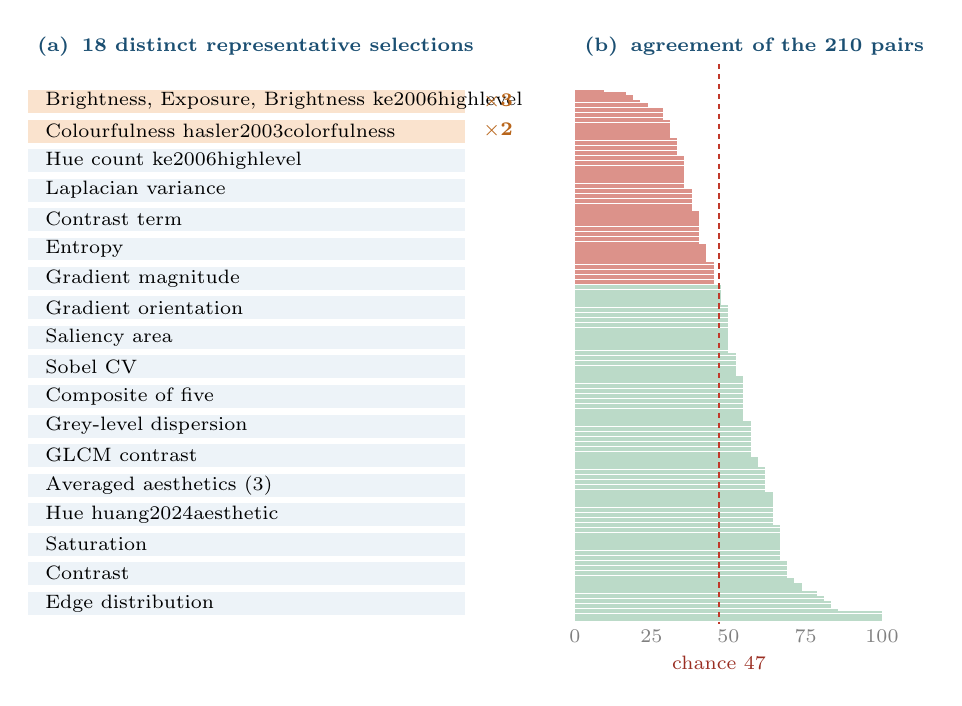
\begin{tikzpicture}[x=1cm,y=1cm,font=\scriptsize]
\node[anchor=west,font=\scriptsize\bfseries,text=headerblue] at (0,0.52) {\textbf{(a)}\enspace18 distinct representative selections};
\fill[accentorange!22] (0,-0.32) rectangle (5.55,-0.03);
\node[anchor=west,font=\scriptsize] at (0.10,-0.17) {Brightness, Exposure, Brightness~\citep{ke2006highlevel}};
\node[anchor=west,font=\scriptsize\bfseries,text=accentorange!80!black] at (5.66,-0.17) {$\times$3};
\fill[accentorange!22] (0,-0.70) rectangle (5.55,-0.41);
\node[anchor=west,font=\scriptsize] at (0.10,-0.55) {Colourfulness~\citep{hasler2003colorfulness}};
\node[anchor=west,font=\scriptsize\bfseries,text=accentorange!80!black] at (5.66,-0.55) {$\times$2};
\fill[rowlight] (0,-1.07) rectangle (5.55,-0.78);
\node[anchor=west,font=\scriptsize] at (0.10,-0.93) {Hue count~\citep{ke2006highlevel}};
\fill[rowlight] (0,-1.45) rectangle (5.55,-1.16);
\node[anchor=west,font=\scriptsize] at (0.10,-1.30) {Laplacian variance};
\fill[rowlight] (0,-1.82) rectangle (5.55,-1.53);
\node[anchor=west,font=\scriptsize] at (0.10,-1.67) {Contrast term};
\fill[rowlight] (0,-2.19) rectangle (5.55,-1.91);
\node[anchor=west,font=\scriptsize] at (0.10,-2.05) {Entropy};
\fill[rowlight] (0,-2.57) rectangle (5.55,-2.28);
\node[anchor=west,font=\scriptsize] at (0.10,-2.43) {Gradient magnitude};
\fill[rowlight] (0,-2.94) rectangle (5.55,-2.65);
\node[anchor=west,font=\scriptsize] at (0.10,-2.80) {Gradient orientation};
\fill[rowlight] (0,-3.32) rectangle (5.55,-3.03);
\node[anchor=west,font=\scriptsize] at (0.10,-3.18) {Saliency area};
\fill[rowlight] (0,-3.69) rectangle (5.55,-3.40);
\node[anchor=west,font=\scriptsize] at (0.10,-3.55) {Sobel CV};
\fill[rowlight] (0,-4.07) rectangle (5.55,-3.78);
\node[anchor=west,font=\scriptsize] at (0.10,-3.93) {Composite of five};
\fill[rowlight] (0,-4.45) rectangle (5.55,-4.16);
\node[anchor=west,font=\scriptsize] at (0.10,-4.30) {Grey-level dispersion};
\fill[rowlight] (0,-4.82) rectangle (5.55,-4.53);
\node[anchor=west,font=\scriptsize] at (0.10,-4.67) {GLCM contrast};
\fill[rowlight] (0,-5.20) rectangle (5.55,-4.91);
\node[anchor=west,font=\scriptsize] at (0.10,-5.05) {Averaged aesthetics (3)};
\fill[rowlight] (0,-5.57) rectangle (5.55,-5.28);
\node[anchor=west,font=\scriptsize] at (0.10,-5.42) {Hue~\citep{huang2024aesthetic}};
\fill[rowlight] (0,-5.95) rectangle (5.55,-5.66);
\node[anchor=west,font=\scriptsize] at (0.10,-5.80) {Saturation};
\fill[rowlight] (0,-6.32) rectangle (5.55,-6.03);
\node[anchor=west,font=\scriptsize] at (0.10,-6.17) {Contrast};
\fill[rowlight] (0,-6.70) rectangle (5.55,-6.41);
\node[anchor=west,font=\scriptsize] at (0.10,-6.55) {Edge distribution};
\node[anchor=west,font=\scriptsize\bfseries,text=headerblue] at (6.95,0.52) {\textbf{(b)}\enspace agreement of the 210 pairs};
\fill[accentred!55] (6.95,-0.058) rectangle (7.32,-0.030);
\fill[accentred!55] (6.95,-0.090) rectangle (7.60,-0.062);
\fill[accentred!55] (6.95,-0.122) rectangle (7.69,-0.094);
\fill[accentred!55] (6.95,-0.154) rectangle (7.69,-0.126);
\fill[accentred!55] (6.95,-0.187) rectangle (7.78,-0.159);
\fill[accentred!55] (6.95,-0.219) rectangle (7.88,-0.191);
\fill[accentred!55] (6.95,-0.251) rectangle (7.88,-0.223);
\fill[accentred!55] (6.95,-0.283) rectangle (8.07,-0.255);
\fill[accentred!55] (6.95,-0.315) rectangle (8.07,-0.287);
\fill[accentred!55] (6.95,-0.347) rectangle (8.07,-0.319);
\fill[accentred!55] (6.95,-0.379) rectangle (8.07,-0.351);
\fill[accentred!55] (6.95,-0.412) rectangle (8.07,-0.384);
\fill[accentred!55] (6.95,-0.444) rectangle (8.16,-0.416);
\fill[accentred!55] (6.95,-0.476) rectangle (8.16,-0.448);
\fill[accentred!55] (6.95,-0.508) rectangle (8.16,-0.480);
\fill[accentred!55] (6.95,-0.540) rectangle (8.16,-0.512);
\fill[accentred!55] (6.95,-0.572) rectangle (8.16,-0.544);
\fill[accentred!55] (6.95,-0.604) rectangle (8.16,-0.576);
\fill[accentred!55] (6.95,-0.637) rectangle (8.16,-0.609);
\fill[accentred!55] (6.95,-0.669) rectangle (8.25,-0.641);
\fill[accentred!55] (6.95,-0.701) rectangle (8.25,-0.673);
\fill[accentred!55] (6.95,-0.733) rectangle (8.25,-0.705);
\fill[accentred!55] (6.95,-0.765) rectangle (8.25,-0.737);
\fill[accentred!55] (6.95,-0.797) rectangle (8.25,-0.769);
\fill[accentred!55] (6.95,-0.829) rectangle (8.25,-0.801);
\fill[accentred!55] (6.95,-0.862) rectangle (8.25,-0.834);
\fill[accentred!55] (6.95,-0.894) rectangle (8.34,-0.866);
\fill[accentred!55] (6.95,-0.926) rectangle (8.34,-0.898);
\fill[accentred!55] (6.95,-0.958) rectangle (8.34,-0.930);
\fill[accentred!55] (6.95,-0.990) rectangle (8.34,-0.962);
\fill[accentred!55] (6.95,-1.022) rectangle (8.34,-0.994);
\fill[accentred!55] (6.95,-1.054) rectangle (8.34,-1.026);
\fill[accentred!55] (6.95,-1.087) rectangle (8.34,-1.059);
\fill[accentred!55] (6.95,-1.119) rectangle (8.34,-1.091);
\fill[accentred!55] (6.95,-1.151) rectangle (8.34,-1.123);
\fill[accentred!55] (6.95,-1.183) rectangle (8.34,-1.155);
\fill[accentred!55] (6.95,-1.215) rectangle (8.34,-1.187);
\fill[accentred!55] (6.95,-1.247) rectangle (8.34,-1.219);
\fill[accentred!55] (6.95,-1.279) rectangle (8.34,-1.251);
\fill[accentred!55] (6.95,-1.312) rectangle (8.44,-1.284);
\fill[accentred!55] (6.95,-1.344) rectangle (8.44,-1.316);
\fill[accentred!55] (6.95,-1.376) rectangle (8.44,-1.348);
\fill[accentred!55] (6.95,-1.408) rectangle (8.44,-1.380);
\fill[accentred!55] (6.95,-1.440) rectangle (8.44,-1.412);
\fill[accentred!55] (6.95,-1.472) rectangle (8.44,-1.444);
\fill[accentred!55] (6.95,-1.504) rectangle (8.44,-1.476);
\fill[accentred!55] (6.95,-1.537) rectangle (8.44,-1.509);
\fill[accentred!55] (6.95,-1.569) rectangle (8.44,-1.541);
\fill[accentred!55] (6.95,-1.601) rectangle (8.53,-1.573);
\fill[accentred!55] (6.95,-1.633) rectangle (8.53,-1.605);
\fill[accentred!55] (6.95,-1.665) rectangle (8.53,-1.637);
\fill[accentred!55] (6.95,-1.697) rectangle (8.53,-1.669);
\fill[accentred!55] (6.95,-1.729) rectangle (8.53,-1.701);
\fill[accentred!55] (6.95,-1.762) rectangle (8.53,-1.734);
\fill[accentred!55] (6.95,-1.794) rectangle (8.53,-1.766);
\fill[accentred!55] (6.95,-1.826) rectangle (8.53,-1.798);
\fill[accentred!55] (6.95,-1.858) rectangle (8.53,-1.830);
\fill[accentred!55] (6.95,-1.890) rectangle (8.53,-1.862);
\fill[accentred!55] (6.95,-1.922) rectangle (8.53,-1.894);
\fill[accentred!55] (6.95,-1.954) rectangle (8.53,-1.926);
\fill[accentred!55] (6.95,-1.987) rectangle (8.53,-1.959);
\fill[accentred!55] (6.95,-2.019) rectangle (8.62,-1.991);
\fill[accentred!55] (6.95,-2.051) rectangle (8.62,-2.023);
\fill[accentred!55] (6.95,-2.083) rectangle (8.62,-2.055);
\fill[accentred!55] (6.95,-2.115) rectangle (8.62,-2.087);
\fill[accentred!55] (6.95,-2.147) rectangle (8.62,-2.119);
\fill[accentred!55] (6.95,-2.179) rectangle (8.62,-2.151);
\fill[accentred!55] (6.95,-2.212) rectangle (8.62,-2.184);
\fill[accentred!55] (6.95,-2.244) rectangle (8.71,-2.216);
\fill[accentred!55] (6.95,-2.276) rectangle (8.71,-2.248);
\fill[accentred!55] (6.95,-2.308) rectangle (8.71,-2.280);
\fill[accentred!55] (6.95,-2.340) rectangle (8.71,-2.312);
\fill[accentred!55] (6.95,-2.372) rectangle (8.71,-2.344);
\fill[accentred!55] (6.95,-2.404) rectangle (8.71,-2.376);
\fill[accentred!55] (6.95,-2.437) rectangle (8.71,-2.409);
\fill[accentred!55] (6.95,-2.469) rectangle (8.71,-2.441);
\fill[accentred!55] (6.95,-2.501) rectangle (8.71,-2.473);
\fill[accentgreen!30] (6.95,-2.533) rectangle (8.81,-2.505);
\fill[accentgreen!30] (6.95,-2.565) rectangle (8.81,-2.537);
\fill[accentgreen!30] (6.95,-2.597) rectangle (8.81,-2.569);
\fill[accentgreen!30] (6.95,-2.629) rectangle (8.81,-2.601);
\fill[accentgreen!30] (6.95,-2.662) rectangle (8.81,-2.634);
\fill[accentgreen!30] (6.95,-2.694) rectangle (8.81,-2.666);
\fill[accentgreen!30] (6.95,-2.726) rectangle (8.81,-2.698);
\fill[accentgreen!30] (6.95,-2.758) rectangle (8.81,-2.730);
\fill[accentgreen!30] (6.95,-2.790) rectangle (8.90,-2.762);
\fill[accentgreen!30] (6.95,-2.822) rectangle (8.90,-2.794);
\fill[accentgreen!30] (6.95,-2.854) rectangle (8.90,-2.826);
\fill[accentgreen!30] (6.95,-2.887) rectangle (8.90,-2.859);
\fill[accentgreen!30] (6.95,-2.919) rectangle (8.90,-2.891);
\fill[accentgreen!30] (6.95,-2.951) rectangle (8.90,-2.923);
\fill[accentgreen!30] (6.95,-2.983) rectangle (8.90,-2.955);
\fill[accentgreen!30] (6.95,-3.015) rectangle (8.90,-2.987);
\fill[accentgreen!30] (6.95,-3.047) rectangle (8.90,-3.019);
\fill[accentgreen!30] (6.95,-3.079) rectangle (8.90,-3.051);
\fill[accentgreen!30] (6.95,-3.112) rectangle (8.90,-3.084);
\fill[accentgreen!30] (6.95,-3.144) rectangle (8.90,-3.116);
\fill[accentgreen!30] (6.95,-3.176) rectangle (8.90,-3.148);
\fill[accentgreen!30] (6.95,-3.208) rectangle (8.90,-3.180);
\fill[accentgreen!30] (6.95,-3.240) rectangle (8.90,-3.212);
\fill[accentgreen!30] (6.95,-3.272) rectangle (8.90,-3.244);
\fill[accentgreen!30] (6.95,-3.304) rectangle (8.90,-3.276);
\fill[accentgreen!30] (6.95,-3.337) rectangle (8.90,-3.309);
\fill[accentgreen!30] (6.95,-3.369) rectangle (8.90,-3.341);
\fill[accentgreen!30] (6.95,-3.401) rectangle (8.99,-3.373);
\fill[accentgreen!30] (6.95,-3.433) rectangle (8.99,-3.405);
\fill[accentgreen!30] (6.95,-3.465) rectangle (8.99,-3.437);
\fill[accentgreen!30] (6.95,-3.497) rectangle (8.99,-3.469);
\fill[accentgreen!30] (6.95,-3.529) rectangle (8.99,-3.501);
\fill[accentgreen!30] (6.95,-3.562) rectangle (8.99,-3.534);
\fill[accentgreen!30] (6.95,-3.594) rectangle (8.99,-3.566);
\fill[accentgreen!30] (6.95,-3.626) rectangle (8.99,-3.598);
\fill[accentgreen!30] (6.95,-3.658) rectangle (8.99,-3.630);
\fill[accentgreen!30] (6.95,-3.690) rectangle (9.09,-3.662);
\fill[accentgreen!30] (6.95,-3.722) rectangle (9.09,-3.694);
\fill[accentgreen!30] (6.95,-3.754) rectangle (9.09,-3.726);
\fill[accentgreen!30] (6.95,-3.787) rectangle (9.09,-3.759);
\fill[accentgreen!30] (6.95,-3.819) rectangle (9.09,-3.791);
\fill[accentgreen!30] (6.95,-3.851) rectangle (9.09,-3.823);
\fill[accentgreen!30] (6.95,-3.883) rectangle (9.09,-3.855);
\fill[accentgreen!30] (6.95,-3.915) rectangle (9.09,-3.887);
\fill[accentgreen!30] (6.95,-3.947) rectangle (9.09,-3.919);
\fill[accentgreen!30] (6.95,-3.979) rectangle (9.09,-3.951);
\fill[accentgreen!30] (6.95,-4.012) rectangle (9.09,-3.984);
\fill[accentgreen!30] (6.95,-4.044) rectangle (9.09,-4.016);
\fill[accentgreen!30] (6.95,-4.076) rectangle (9.09,-4.048);
\fill[accentgreen!30] (6.95,-4.108) rectangle (9.09,-4.080);
\fill[accentgreen!30] (6.95,-4.140) rectangle (9.09,-4.112);
\fill[accentgreen!30] (6.95,-4.172) rectangle (9.09,-4.144);
\fill[accentgreen!30] (6.95,-4.204) rectangle (9.09,-4.176);
\fill[accentgreen!30] (6.95,-4.237) rectangle (9.09,-4.209);
\fill[accentgreen!30] (6.95,-4.269) rectangle (9.18,-4.241);
\fill[accentgreen!30] (6.95,-4.301) rectangle (9.18,-4.273);
\fill[accentgreen!30] (6.95,-4.333) rectangle (9.18,-4.305);
\fill[accentgreen!30] (6.95,-4.365) rectangle (9.18,-4.337);
\fill[accentgreen!30] (6.95,-4.397) rectangle (9.18,-4.369);
\fill[accentgreen!30] (6.95,-4.429) rectangle (9.18,-4.401);
\fill[accentgreen!30] (6.95,-4.462) rectangle (9.18,-4.434);
\fill[accentgreen!30] (6.95,-4.494) rectangle (9.18,-4.466);
\fill[accentgreen!30] (6.95,-4.526) rectangle (9.18,-4.498);
\fill[accentgreen!30] (6.95,-4.558) rectangle (9.18,-4.530);
\fill[accentgreen!30] (6.95,-4.590) rectangle (9.18,-4.562);
\fill[accentgreen!30] (6.95,-4.622) rectangle (9.18,-4.594);
\fill[accentgreen!30] (6.95,-4.654) rectangle (9.18,-4.626);
\fill[accentgreen!30] (6.95,-4.687) rectangle (9.18,-4.659);
\fill[accentgreen!30] (6.95,-4.719) rectangle (9.27,-4.691);
\fill[accentgreen!30] (6.95,-4.751) rectangle (9.27,-4.723);
\fill[accentgreen!30] (6.95,-4.783) rectangle (9.27,-4.755);
\fill[accentgreen!30] (6.95,-4.815) rectangle (9.27,-4.787);
\fill[accentgreen!30] (6.95,-4.847) rectangle (9.36,-4.819);
\fill[accentgreen!30] (6.95,-4.879) rectangle (9.36,-4.851);
\fill[accentgreen!30] (6.95,-4.912) rectangle (9.36,-4.884);
\fill[accentgreen!30] (6.95,-4.944) rectangle (9.36,-4.916);
\fill[accentgreen!30] (6.95,-4.976) rectangle (9.36,-4.948);
\fill[accentgreen!30] (6.95,-5.008) rectangle (9.36,-4.980);
\fill[accentgreen!30] (6.95,-5.040) rectangle (9.36,-5.012);
\fill[accentgreen!30] (6.95,-5.072) rectangle (9.36,-5.044);
\fill[accentgreen!30] (6.95,-5.104) rectangle (9.36,-5.076);
\fill[accentgreen!30] (6.95,-5.137) rectangle (9.36,-5.109);
\fill[accentgreen!30] (6.95,-5.169) rectangle (9.46,-5.141);
\fill[accentgreen!30] (6.95,-5.201) rectangle (9.46,-5.173);
\fill[accentgreen!30] (6.95,-5.233) rectangle (9.46,-5.205);
\fill[accentgreen!30] (6.95,-5.265) rectangle (9.46,-5.237);
\fill[accentgreen!30] (6.95,-5.297) rectangle (9.46,-5.269);
\fill[accentgreen!30] (6.95,-5.329) rectangle (9.46,-5.301);
\fill[accentgreen!30] (6.95,-5.362) rectangle (9.46,-5.334);
\fill[accentgreen!30] (6.95,-5.394) rectangle (9.46,-5.366);
\fill[accentgreen!30] (6.95,-5.426) rectangle (9.46,-5.398);
\fill[accentgreen!30] (6.95,-5.458) rectangle (9.46,-5.430);
\fill[accentgreen!30] (6.95,-5.490) rectangle (9.46,-5.462);
\fill[accentgreen!30] (6.95,-5.522) rectangle (9.46,-5.494);
\fill[accentgreen!30] (6.95,-5.554) rectangle (9.46,-5.526);
\fill[accentgreen!30] (6.95,-5.587) rectangle (9.55,-5.559);
\fill[accentgreen!30] (6.95,-5.619) rectangle (9.55,-5.591);
\fill[accentgreen!30] (6.95,-5.651) rectangle (9.55,-5.623);
\fill[accentgreen!30] (6.95,-5.683) rectangle (9.55,-5.655);
\fill[accentgreen!30] (6.95,-5.715) rectangle (9.55,-5.687);
\fill[accentgreen!30] (6.95,-5.747) rectangle (9.55,-5.719);
\fill[accentgreen!30] (6.95,-5.779) rectangle (9.55,-5.751);
\fill[accentgreen!30] (6.95,-5.812) rectangle (9.55,-5.784);
\fill[accentgreen!30] (6.95,-5.844) rectangle (9.55,-5.816);
\fill[accentgreen!30] (6.95,-5.876) rectangle (9.55,-5.848);
\fill[accentgreen!30] (6.95,-5.908) rectangle (9.55,-5.880);
\fill[accentgreen!30] (6.95,-5.940) rectangle (9.55,-5.912);
\fill[accentgreen!30] (6.95,-5.972) rectangle (9.55,-5.944);
\fill[accentgreen!30] (6.95,-6.004) rectangle (9.55,-5.976);
\fill[accentgreen!30] (6.95,-6.037) rectangle (9.64,-6.009);
\fill[accentgreen!30] (6.95,-6.069) rectangle (9.64,-6.041);
\fill[accentgreen!30] (6.95,-6.101) rectangle (9.64,-6.073);
\fill[accentgreen!30] (6.95,-6.133) rectangle (9.64,-6.105);
\fill[accentgreen!30] (6.95,-6.165) rectangle (9.64,-6.137);
\fill[accentgreen!30] (6.95,-6.197) rectangle (9.64,-6.169);
\fill[accentgreen!30] (6.95,-6.229) rectangle (9.64,-6.201);
\fill[accentgreen!30] (6.95,-6.262) rectangle (9.73,-6.234);
\fill[accentgreen!30] (6.95,-6.294) rectangle (9.73,-6.266);
\fill[accentgreen!30] (6.95,-6.326) rectangle (9.83,-6.298);
\fill[accentgreen!30] (6.95,-6.358) rectangle (9.83,-6.330);
\fill[accentgreen!30] (6.95,-6.390) rectangle (9.83,-6.362);
\fill[accentgreen!30] (6.95,-6.422) rectangle (10.02,-6.394);
\fill[accentgreen!30] (6.95,-6.454) rectangle (10.02,-6.426);
\fill[accentgreen!30] (6.95,-6.487) rectangle (10.11,-6.459);
\fill[accentgreen!30] (6.95,-6.519) rectangle (10.11,-6.491);
\fill[accentgreen!30] (6.95,-6.551) rectangle (10.20,-6.523);
\fill[accentgreen!30] (6.95,-6.583) rectangle (10.20,-6.555);
\fill[accentgreen!30] (6.95,-6.615) rectangle (10.20,-6.587);
\fill[accentgreen!30] (6.95,-6.647) rectangle (10.29,-6.619);
\fill[accentgreen!30] (6.95,-6.679) rectangle (10.85,-6.651);
\fill[accentgreen!30] (6.95,-6.712) rectangle (10.85,-6.684);
\fill[accentgreen!30] (6.95,-6.744) rectangle (10.85,-6.716);
\fill[accentgreen!30] (6.95,-6.776) rectangle (10.85,-6.748);
\node[font=\scriptsize,text=black!50] at (6.95,-6.97) {0};
\node[font=\scriptsize,text=black!50] at (7.92,-6.97) {25};
\node[font=\scriptsize,text=black!50] at (8.90,-6.97) {50};
\node[font=\scriptsize,text=black!50] at (9.88,-6.97) {75};
\node[font=\scriptsize,text=black!50] at (10.85,-6.97) {100};
\draw[accentred,line width=.8pt,dash pattern=on 2pt off 1.6pt] (8.78,0.30) -- (8.78,-6.81);
\node[anchor=north,font=\scriptsize,text=accentred!80!black] at (8.78,-7.09) {chance 47};
\end{tikzpicture}
\caption{The same 42 redundancy clusters and the same pipeline, with only the visual-selection operation swapped; \textbf{no reference model is involved}. \textbf{(a)}: the twenty-one operations grouped by the representative set each produces, giving eighteen \emph{distinct sets}; a group of more than one operation carries its size as a multiplier. \textbf{(b)}: agreement for each of the 210 \emph{unordered operation pairs}, sorted, against the chance floor of $47$ per cent (dashed); \textbf{77 pairs agree below chance}. The only groups that agree completely are operations computing the same quantity: the brightness variants and the two colourfulness implementations. \textbf{SIFT+BoVW is absent from this panel by design}: every operation here scores the same input regime, and its key-frame selector is part of the published method, so holding the input fixed would evaluate a different operation. The matched-input control of Section~4.6 is the diagnostic that compares it under a common interface. \emph{Labels}: CV, coefficient of variation; GLCM, grey-level co-occurrence matrix. Rows that name the same attribute carry the reference of the work that defines it.}
\label{fig:menu}
\end{figure}


Read against one fixed choice, the same swaps rewrite much of the stage output
(Figure~S4): of the \jusTotal{} alternatives, \jusAbaixo{} retain less than chance.
\textbf{That comparison shares the clusters but not the frames}: the per-frame operations
score one frame per second, while SIFT+BoVW runs its own key-frame selector.

%% ⭐ 27/09 (cli-3, alvo de 28 p do Jader): o \FloatBarrier que ficava aqui deixava MEIA
%% pagina vazia antes da Figura 2, porque o texto seguinte nao podia subir enquanto a
%% figura nao saisse. A barreira do fim da 4.7 continua segurando a figura antes da 5.
LIQE was used for the complete-implementation substitution, having the largest
generalization margin among the three eligible methods. The substitution changes \casCompleta{} of the 42 representatives, the two operations agreeing in \subResta{} clusters (\subPct{} per cent, 95\% CI \fusIC{} over the \fusBlocos{} source-aware blocks), close to the \subAcaso{} per cent uniform-choice expectation. Whether the substitution also improves the output, measured with the technical branch of DOVER, is model-based evidence reported in the supplement, where for the complete substitution both intervals cross zero.

Under matched inputs the picture sharpens. Given at most ten uniformly spaced
frames, \casQuadrosMedia{} in common on average, and mean pooling for both, SIFT+BoVW and
LIQE still select different representatives in 16 of the 42 clusters.
Holding the scorer fixed while changing only sampling and pooling already moves
\casSoCasamento{} decisions against \casCompleta{} for the complete operation; an exact
McNemar test separates the two regimes ($p=\casP{}$), as does the block sign-flip over the
\mcnBlocos{} topics ($p=\mcnBloco{}$). Both scorer identity and input sampling carry part of the effect.

%% ⚠️ este ponteiro vive longe do da Figura~S4 de proposito: os dois na mesma janela
%% faziam o sincronizador reescrever o numero de um com o do outro.
The retention percentages above put all \disOps{} operations of Figure~\ref{fig:menu}
on one frame per second, which makes their spread attributable to the scorer; Table~S19
scores each complete operation under its own sampling.

\subsection{Source-level synthesis of the audit}\label{sec:synthesis}

Table~\ref{tab:synthesis} brings together the roles the sources document and the results of
the implementations evaluated here, organized by work and component. \textbf{The one audited source that names technical fidelity as the aim of a term}, Ref.~\citep{xu2024property}, implements it with BRISQUE, one of five dimensions of its regret-minimization query; evaluated alone here, BRISQUE does not meet both external conditions.

%% GERADO por gera_tab_sintese.py. Nao editar a mao.
\begin{table}[p]
\caption{\textbf{The audit read by source work.} Each band is one source with the role it declares; each row is one component. \textbf{Degradation columns} give strict accuracy (per cent) on the constructed pairs, \textbf{50 being chance}, green where the operation prefers the original and red where it prefers the degraded copy; every cell prints its value, so the table reads in greyscale. \emph{Dk} darkening, \emph{Mo} motion blur, \emph{Bl} Gaussian blur, \emph{H2} H.264, \emph{Rs} rescaling, \emph{St} desaturation, \emph{Ns} white noise, \emph{Jp} JPEG. \textbf{Mean} is over all eight types, not the seven-type contrast of Section~\ref{sec:combinations}. \textbf{Agr} is chance-corrected agreement with LIQE, the designated reference for the literature-derived operations, over the 42 operational clusters. \textbf{Denominator}: 800 pairs (20 segments $\times$ 8 types $\times$ 5 levels), except the Ref.~\citep{korolkov2025keyframe} band, which runs on the 11 segments carrying both of its inputs and therefore on 440 pairs. $^{*}$ the degradation acts directly on the quantity that operation measures; $^{\dagger}$ the same computation is used by two source works, so the two rows are not independent evidence; $^{\ddagger}$ the same Hasler expression, named by several sources; $^{\S}$ a term of the published module implemented after the inventory freeze, outside the counts each band states; $^{\P}$ audited on the same footing but outside the eleven-work count, because it is the testbed's own operation. $^{\mathrm{m}}$ the one model row: its agreement comes from the common-reference analysis of Section~\ref{sec:screen_results}, which scores both families against LIQE. \emph{n/a} marks a test that does not apply, and \textbf{a dash marks one that applies but was not run}.}
\label{tab:synthesis}
\centering
\tiny
\setlength{\tabcolsep}{2.0pt}
\renewcommand{\arraystretch}{.86}
\begin{tabular}{@{}lcccccccc@{\hskip 4pt}r@{\hskip 4pt}r@{}}
\toprule
& \multicolumn{8}{c}{\textbf{\footnotesize degradation type}} & &\\
\cmidrule(lr){2-9}
\textbf{Source work / component} & \textbf{Dk} & \textbf{Mo} & \textbf{Bl} & \textbf{H2} & \textbf{Rs} & \textbf{St} & \textbf{Ns} & \textbf{Jp} & \textbf{Mean} & \textbf{Agr}\\
\midrule
\rowcolor{headerblue!10}\multicolumn{11}{@{}p{\linewidth}@{}}{Ref.~\citep{ke2006highlevel}\ \textcolor{black!78}{four features of a naive Bayes photo-quality classifier;} \textcolor{black!72}{\itshape here: each feature alone, as a score;} \textcolor{accentblue}{\textbf{human ratings; per feature and combined}}}\\
Edge distribution & \cellcolor{perf4!70}70 & \cellcolor{perf4!70}\textcolor{black!75}{\itshape 62}\rlap{\tiny$^{*}$} & \cellcolor{perf4!70}\textcolor{black!75}{\itshape 62}\rlap{\tiny$^{*}$} & \cellcolor{perf1!70}11 & \cellcolor{perf4!70}74 & \cellcolor{perf5!45}97 & \cellcolor{perf5!45}100 & \cellcolor{perf2!70}31 & \textbf{63.4} & \textcolor{accentred}{\textbf{$-.124$}}\\
Hue count & \cellcolor{perf2!70}20 & \cellcolor{perf1!70}13 & \cellcolor{perf1!70}10 & \cellcolor{perf4!70}77 & \cellcolor{perf1!70}11 & \cellcolor{perf1!70}4 & \cellcolor{perf5!45}100 & \cellcolor{perf3!80}59 & \textbf{36.8} & \textcolor{accentred}{\textbf{$-.258$}}\\
Contrast & \cellcolor{perf5!45}\textcolor{black!75}{\itshape 100}\rlap{\tiny$^{*}$} & \cellcolor{perf5!45}100 & \cellcolor{perf5!45}100 & \cellcolor{perf5!45}98 & \cellcolor{perf5!45}100 & \cellcolor{perf2!70}30 & \cellcolor{perf1!70}10 & \cellcolor{perf4!70}60 & \textbf{74.8} & $+.326$\\
Colourfulness$^{\ddagger}$ & \cellcolor{perf5!45}100 & \cellcolor{perf5!45}100 & \cellcolor{perf5!45}100 & \cellcolor{perf5!45}100 & \cellcolor{perf5!45}100 & \cellcolor{perf5!45}\textcolor{black!75}{\itshape 100}\rlap{\tiny$^{*}$} & \cellcolor{perf1!70}3 & \cellcolor{perf4!70}79 & \textbf{85.2} & $+.281$\\
\rowcolor{headerblue!10}\multicolumn{11}{@{}p{\linewidth}@{}}{Ref.~\citep{srinivas2016rank}\ \textcolor{black!78}{average five attributes into a per-frame quality score;} \textcolor{black!72}{\itshape here: its mean rule, on our attribute vector;} \textcolor{accentblue}{summary-level evaluation}}\\
The mean rule, our vector & \cellcolor{perf5!45}100 & \cellcolor{perf5!45}100 & \cellcolor{perf5!45}100 & \cellcolor{perf5!45}100 & \cellcolor{perf5!45}100 & \cellcolor{perf5!45}98 & \cellcolor{perf2!70}29 & \cellcolor{perf4!70}69 & \textbf{87.0} & $+.371$\\
\rowcolor{headerblue!10}\multicolumn{11}{@{}p{\linewidth}@{}}{Ref.~\citep{qaroush2025diversity}\ \textcolor{black!78}{four audited terms across three objectives, and a five-term attention module;} \textcolor{black!72}{\itshape here: the published rule over the vector implemented here, then each term;} \textcolor{accentblue}{summary-level evaluation}}\\
Visual-attention module & \cellcolor{perf5!45}100 & \cellcolor{perf5!45}100 & \cellcolor{perf5!45}100 & \cellcolor{perf5!45}100 & \cellcolor{perf5!45}100 & \cellcolor{perf5!45}100 & \cellcolor{perf1!70}0 & \cellcolor{perf2!70}20 & \textbf{77.5} & \textcolor{black!30}{\tiny n/a}\\
\quad Colourfulness$^{\ddagger}$ & \cellcolor{perf5!45}100 & \cellcolor{perf5!45}100 & \cellcolor{perf5!45}100 & \cellcolor{perf5!45}100 & \cellcolor{perf5!45}100 & \cellcolor{perf5!45}\textcolor{black!75}{\itshape 100}\rlap{\tiny$^{*}$} & \cellcolor{perf1!70}3 & \cellcolor{perf4!70}79 & \textbf{85.2} & $+.281$\\
\quad Gradient magnitude & \cellcolor{perf5!45}100 & \cellcolor{perf5!45}100 & \cellcolor{perf5!45}100 & \cellcolor{perf5!45}100 & \cellcolor{perf5!45}100 & \cellcolor{perf2!70}23 & \cellcolor{perf1!70}0 & \cellcolor{perf1!70}5 & \textbf{66.0} & $+.551$\\
\quad Saliency & \cellcolor{perf4!70}62 & \cellcolor{perf2!70}29 & \cellcolor{perf2!70}20 & \cellcolor{perf5!45}94 & \cellcolor{perf2!70}21 & \cellcolor{perf1!70}18 & \cellcolor{perf1!70}13 & \cellcolor{perf1!70}10 & \textbf{33.4} & $+.101$\\
\quad Contrast term$^{\S}$ & \cellcolor{perf1!70}0 & \cellcolor{perf1!70}0 & \cellcolor{perf1!70}0 & \cellcolor{perf1!70}3 & \cellcolor{perf1!70}0 & \cellcolor{perf4!70}68 & \cellcolor{perf5!45}81 & \cellcolor{perf3!80}55 & \textbf{25.9} & \textcolor{black!30}{---}\\
\quad Motion magnitude$^{\S}$ & \cellcolor{perf5!45}100 & \cellcolor{perf5!45}87 & \cellcolor{perf5!45}100 & \cellcolor{perf5!45}98 & \cellcolor{perf5!45}98 & \cellcolor{perf1!70}14 & \cellcolor{perf1!70}9 & \cellcolor{perf1!70}10 & \textbf{64.5} & \textcolor{black!30}{---}\\
Entropy & \cellcolor{perf5!45}100 & \cellcolor{perf4!70}77 & \cellcolor{perf5!45}83 & \cellcolor{perf1!70}10 & \cellcolor{perf4!70}77 & \cellcolor{perf5!45}97 & \cellcolor{perf1!70}0 & \cellcolor{perf4!70}66 & \textbf{63.8} & $+.236$\\
Gradient orientation & \cellcolor{perf5!45}100 & \cellcolor{perf5!45}80 & \cellcolor{perf2!70}26 & \cellcolor{perf5!45}95 & \cellcolor{perf1!70}9 & \cellcolor{perf2!70}21 & \cellcolor{perf1!70}0 & \cellcolor{perf5!45}100 & \textbf{53.9} & $+.461$\\
\rowcolor{headerblue!10}\multicolumn{11}{@{}p{\linewidth}@{}}{Ref.~\citep{korolkov2025keyframe}\ \textcolor{black!78}{$.7\,z(\mathrm{sharp})+.3\,z(\mathrm{bright})$ as a keyframe score, \textbf{on 11 of the 20 segments};} \textcolor{black!72}{\itshape here: the rule, our normalization population;} \textcolor{accentblue}{\textbf{no isolated test of the rule}}}\\
The published rule & \cellcolor{perf5!45}100 & \cellcolor{perf5!45}100 & \cellcolor{perf5!45}100 & \cellcolor{perf5!45}100 & \cellcolor{perf5!45}100 & \cellcolor{perf1!70}0 & \cellcolor{perf1!70}0 & \cellcolor{perf3!80}49 & \textbf{68.6} & \textcolor{black!30}{\tiny n/a}\\
\quad Sharpness alone, same 11$^{\dagger}$ & \cellcolor{perf5!45}100 & \cellcolor{perf5!45}100 & \cellcolor{perf5!45}100 & \cellcolor{perf5!45}91 & \cellcolor{perf5!45}100 & \cellcolor{perf3!80}47 & \cellcolor{perf1!70}0 & \cellcolor{perf3!80}49 & \textbf{73.4} & \textcolor{black!30}{\tiny n/a}\\
\rowcolor{headerblue!10}\multicolumn{11}{@{}p{\linewidth}@{}}{Ref.~\citep{cakmak2025tripss}\ \textcolor{black!78}{a threshold discarding blurred frames, not a score;} \textcolor{black!72}{\itshape here: the statistic as a scorer, not the filter;} \textcolor{accentblue}{summary-level evaluation, with ablation}}\\
Laplacian variance$^{\dagger}$ & \cellcolor{perf5!45}100 & \cellcolor{perf5!45}\textcolor{black!75}{\itshape 100}\rlap{\tiny$^{*}$} & \cellcolor{perf5!45}\textcolor{black!75}{\itshape 100}\rlap{\tiny$^{*}$} & \cellcolor{perf5!45}95 & \cellcolor{perf5!45}100 & \cellcolor{perf3!80}50 & \cellcolor{perf1!70}0 & \cellcolor{perf4!70}66 & \textbf{76.4} & $+.506$\\
\rowcolor{headerblue!10}\multicolumn{11}{@{}p{\linewidth}@{}}{Ref.~\citep{jeong2016static}\ \textcolor{black!78}{a badness term in a cost multiplicative in cluster distance;} \textcolor{black!72}{\itshape here: the term, read increasing;} \textcolor{accentblue}{summary-level evaluation, with an optimisation ablation}}\\
Grey-level dispersion$^{\dagger}$ & \cellcolor{perf5!45}\textcolor{black!75}{\itshape 100}\rlap{\tiny$^{*}$} & \cellcolor{perf5!45}100 & \cellcolor{perf5!45}100 & \cellcolor{perf5!45}100 & \cellcolor{perf5!45}100 & \cellcolor{perf2!70}22 & \cellcolor{perf2!70}25 & \cellcolor{perf5!45}90 & \textbf{79.6} & $+.191$\\
\rowcolor{headerblue!10}\multicolumn{11}{@{}p{\linewidth}@{}}{Ref.~\citep{xu2024property}\ \textcolor{black!78}{a discard filter for meaningless frames, and BRISQUE as one of five score dimensions;} \textcolor{black!72}{\itshape here: the filter statistic and the fidelity dimension, read alone;} \textcolor{accentblue}{summary-level evaluation, with ablation}}\\
Grey-level dispersion$^{\dagger}$ & \cellcolor{perf5!45}\textcolor{black!75}{\itshape 100}\rlap{\tiny$^{*}$} & \cellcolor{perf5!45}100 & \cellcolor{perf5!45}100 & \cellcolor{perf5!45}100 & \cellcolor{perf5!45}100 & \cellcolor{perf2!70}22 & \cellcolor{perf2!70}25 & \cellcolor{perf5!45}90 & \textbf{79.6} & $+.191$\\
\quad BRISQUE, the fidelity dimension$^{\mathrm{m}}$ & \cellcolor{perf5!45}100 & \cellcolor{perf5!45}100 & \cellcolor{perf5!45}100 & \cellcolor{perf5!45}99 & \cellcolor{perf5!45}100 & \cellcolor{perf1!70}0 & \cellcolor{perf4!70}67 & \cellcolor{perf5!45}80 & \textbf{80.8} & $+.685$\\
\rowcolor{headerblue!10}\multicolumn{11}{@{}p{\linewidth}@{}}{Ref.~\citep{barbieri2021tese}$^{\P}$\ \textcolor{black!78}{a TF-IDF sum over a visual-word vocabulary, scoring whether a segment holds images of interest (a relevance criterion);} \textcolor{black!72}{\itshape here: the score as the source specifies it;} \textcolor{accentblue}{\textit{the testbed's own operation}}}\\
SIFT$+$BoVW sum$^{\P}$ & \cellcolor{perf5!45}100 & \cellcolor{perf5!45}100 & \cellcolor{perf5!45}90 & \cellcolor{perf5!45}90 & \cellcolor{perf5!45}88 & \cellcolor{perf2!70}39 & \cellcolor{perf1!70}8 & \cellcolor{perf1!70}6 & \textbf{65.1} & $+.011$\\
\rowcolor{headerblue!10}\multicolumn{11}{@{}p{\linewidth}@{}}{Ref.~\citep{yang2024keyframe}\ \textcolor{black!78}{one texture term of several;} \textcolor{black!72}{\itshape here: the term alone;} \textcolor{accentblue}{summary-level evaluation, with ablation}}\\
GLCM contrast & \cellcolor{perf5!45}100 & \cellcolor{perf5!45}100 & \cellcolor{perf5!45}100 & \cellcolor{perf5!45}100 & \cellcolor{perf5!45}100 & \cellcolor{perf4!70}67 & \cellcolor{perf1!70}0 & \cellcolor{perf4!70}72 & \textbf{79.9} & $+.461$\\
\rowcolor{headerblue!10}\multicolumn{11}{@{}p{\linewidth}@{}}{Ref.~\citep{huang2024aesthetic}\ \textcolor{black!78}{one aesthetic attribute of several;} \textcolor{black!72}{\itshape here: the attribute alone;} \textcolor{accentblue}{summary-level evaluation}}\\
Saturation & \cellcolor{perf1!70}13 & \cellcolor{perf5!45}100 & \cellcolor{perf5!45}100 & \cellcolor{perf1!70}15 & \cellcolor{perf5!45}100 & \cellcolor{perf5!45}\textcolor{black!75}{\itshape 100}\rlap{\tiny$^{*}$} & \cellcolor{perf1!70}1 & \cellcolor{perf5!45}90 & \textbf{64.9} & $+.011$\\
\rowcolor{headerblue!10}\multicolumn{11}{@{}p{\linewidth}@{}}{Ref.~\citep{gygli2014summe}\ \textcolor{black!78}{three aesthetic attributes, listed without a combination;} \textcolor{black!72}{\itshape here: the raw mean;} \textcolor{accentblue}{summary-level evaluation, with ablation}}\\
Averaged aesthetics & \cellcolor{perf5!45}100 & \cellcolor{perf5!45}100 & \cellcolor{perf5!45}100 & \cellcolor{perf5!45}100 & \cellcolor{perf5!45}100 & \cellcolor{perf5!45}100 & \cellcolor{perf1!70}3 & \cellcolor{perf4!70}67 & \textbf{83.8} & $+.461$\\
\rowcolor{headerblue!10}\multicolumn{11}{@{}p{\linewidth}@{}}{Ref.~\citep{hasler2003colorfulness}\ \textcolor{black!78}{\textbf{the one autonomous index}, and it indexes colourfulness;} \textcolor{black!72}{\itshape here: the index as published;} \textcolor{accentblue}{\textbf{human ratings of the named property}}}\\
Colourfulness$^{\ddagger}$ & \cellcolor{perf5!45}100 & \cellcolor{perf5!45}100 & \cellcolor{perf5!45}100 & \cellcolor{perf5!45}100 & \cellcolor{perf5!45}100 & \cellcolor{perf5!45}\textcolor{black!75}{\itshape 100}\rlap{\tiny$^{*}$} & \cellcolor{perf1!70}3 & \cellcolor{perf4!70}79 & \textbf{85.2} & $+.281$\\
\bottomrule
\end{tabular}
\end{table}



%% ⛔ 21/09 (parecer, E71, criterios 7, 8, 9, 20, 35, 47): o denominador \acvPdfs{} e o
%% ACERVO INTEIRO — textos, IQA e sumarizadores —, nao o conjunto elegivel, e «nao citar
%% modelo dedicado» nao demonstra que o trabalho use uma operacao no lugar nem que
%% pretenda medir qualidade tecnica. A ausencia de citacao deixa de sustentar inferencia
%% de substituicao ou de intencao; ficam os casos documentados.
Three patterns emerge in the sources read in full: attribute borrowing, role
reassignment, and summary-level validation. The counts are of confirmed uses, each with a verbatim excerpt.

\emph{Role reassignment} shows the same computation carrying different claims. Laplacian
variance appears as a threshold discarding blurred frames in Ref.~\citep{cakmak2025tripss} and as the dominant weighted term of a keyframe score in Ref.~\citep{korolkov2025keyframe}. What
was measured is the statistic \emph{as a scorer}: it answers blur on every pair and
inverts under noise. The published threshold was not run: a scorer can order a pair correctly while a threshold keeps or drops both members.

\emph{Attribute borrowing} and the level of validation are read from each source. Of the
\valComPdf{} works whose full text is in the archive, \valPropriedade{} test a measure
against human judgement of the property it names, evidence for a different construct: neither validates a single attribute as a stand-alone
score of technical fidelity. By the provenance rule of Section~\ref{sec:prov},
\autAutonomas{} of the \autVerificadas{} operations is a stand-alone index in its
source, and it indexes colourfulness rather than quality; the rest enter as classifier
features, terms of a sum, or signals in a discard filter. Among the remaining works,
\valSoResumo{} report summary-level evaluation, which does not isolate the component's
validity, and the \valSemTeste{} left reports no isolated test of its own rule or
weights, so the three categories account for all \valComPdf{}.



%% ⚠️ 28/09 (cli-3): a barreira que segurava a Tabela 6 aqui deixava meia pagina vazia no fim
%% da 4.7 e levou o corpo a 29 p. Ela foi para antes da 5.1, na discussao: a Tabela 6 continua
%% sem escapar para depois das referencias.

\section{Discussion and limitations}\label{sec:discussion}

%% ⛔ PROSA SUBSTITUIDA em 04/10/2026 pelo texto do Prof. Rudinei (e-mail ao Jader): secao
%% corrida, sem a subsecao Limitations, e sem parte das autocriticas, que ele tirou de
%% proposito («ou vao confundir o revisor ou ja sao esperadas»). NAO restaurar as autocriticas.
%% Aplicada com quatro ajustes, decididos pelo Jader em 04/10, que mudam o que o texto AFIRMA:
%%  1. «keypoint density» -> «descriptor count»: a fatoracao e em D_i, e keypoint density e
%%     outro controle diagnostico do Metodo (sec_method, controles diagnosticos).
%%  2. o ruido nas OUTRAS operacoes fica como consistencia, nao causa: o mecanismo so e medido
%%     no SIFT+BoVW, e a Conclusao diz «measured for that score and consistent with the others».
%%  3. a citacao do Otani e o ponteiro as Tabelas S24 e S25 voltaram.
%%  4. sem «across hardware runs» (causa que o artigo nao afirma) e «later», nao «prospective».
%%  5. «visual quality» saiu duas vezes (convencao de termos de 08/09).
%% Os numeros que ja eram macro continuam macro.

The central finding of this study is that visual-selection statistics derived from the video summarization literature, when reused as standalone technical-quality scores, fail to satisfy the technical-fidelity requirements proposed here. The algebraic factorization of the SIFT+BoVW raw-count score demonstrates that its behavior is overwhelmingly driven by descriptor count rather than visual fidelity; replacing the score with the raw descriptor count preserves every single choice across the \redDe{} operational clusters. For other operations, the concentration of reversals under white noise is consistent with noise inflating local high-frequency detail, which these statistics can misread as superior quality. At the application level, our evaluation separates scoring behavior from output preference, establishing selection sensitivity rather than guaranteeing product improvement. Consequently, practical reuses of these operations require explicit documentation of the intended property, exact statistics, declared polarity, sampling, and aggregation regimes. Although dedicated no-reference image quality assessment (NR-IQA) models offer better-supported alternatives, their robustness remains tightly bound to training exposure, distortion types, and domain characteristics. These findings reframe two readings in the current literature: first, extending the evaluation-side insight of Ref.~\citep{otani2019rethinking}, that protocol choices can dominate summarization scores, to the selection stage; and second, showing that isolated visual attributes frequently fail when extracted from the broader objective functions in which they were originally embedded.

These conclusions must be interpreted alongside some inherent limitations. First, while the quantitative measurements are fully deterministic given the benchmark inventory, the upstream process of compiling the archive, coding each source's functional role, and recording validation evidence relied on manual analysis by a single author. To ensure reproducibility and verification, all \valComPdf{} source works were read in full, and every attribution is anchored to recorded verbatim excerpts (Tables~S24 and~S25). Furthermore, our experimental scope is restricted to selected implementations across three image-quality databases and one broadcast-news pipeline; as a result, these conclusions do not automatically extend to different tasks, model families, or newer neural checkpoints.

The design of the benchmark and inference protocols also introduces specific constraints. The constructed evaluation benchmark comprises twenty video segments organized into \invBlocosN{} source-aware blocks, where ground-truth fidelity is established via controlled algorithmic transformations rather than subjective human preference. Statistical inference remains sensitive to small-sample tail conventions and spatial dependence assumptions, particularly given that eligibility thresholds and most inference parameters were not preregistered. Consequently, analytical variations such as best-component contrasts, oracle polarity alignment, and in-sample ridge regressions serve purely as diagnostic insights rather than prospective validations.

At the operational application level, the 42 redundancy clusters represent operationally redundant segment alternatives nested across 19 news topics with shared source material, rather than strictly semantically equivalent recordings. Because no human subjective quality ratings were collected for these specific segments, the reference benchmarks evaluate response to controlled signal degradation rather than human preference between distinct video captures. Technical quality here functions strictly as a tie-breaker within redundancy groups rather than a holistic verdict on the resulting summary. Similarly, external DOVER comparisons cannot isolate temporal modeling effects from underlying neural architecture or training data, and the official standardized fusion model was omitted.

Finally, the auxiliary diagnostic analyses presented are descriptive rather than confirmatory. In particular, conditioning the SIFT+BoVW score directly on keypoint counts risks removing legitimate quality signals alongside the dominant count channel. While the archived execution outputs allow full reconstruction of all derived statistics, the original software execution environment is not bit-identical. Lastly, partial-coverage models and later deep control architectures remain outside the primary screening comparisons evaluated in this audit.

\section{Conclusion}\label{sec:conclusion}

%% ⛔ PROSA SUBSTITUIDA em 25/09/2026 (item 16). Os numeros continuam todos em macro.
Visual-selection operations from the summarization literature, reused as standalone
technical-quality scores, fail in that role, and the choice among them changes what a
pipeline selects. Every one of the \fontesDaLiteratura{} directionally
specified operations prefers the degraded copy on at least one controlled transformation,
\invOpsSigTop{} keep that reversal under the most conservative analysis, and none of them,
nor any of the \resCombinacoes{} attribute configurations, meets both external screening
conditions; \resElegiveis{} of \invModelos{} dedicated NR-IQA models do. At \taxCentPar{} per cent the deep proxy sits below \taxCentAbaixoDe{} of the \fontesDaLiteratura{} literature operations and below every dedicated model; most of that survives when the cluster members come from other topics, so what it detects is a copy made atypical by degradation, which is representativeness standing in for quality.

The failures share a pattern. Under white noise, the one transformation that adds local high-frequency content,
\resRuido{} of the \fontesDaLiteratura{} operations reverse, and for
the one audited score whose terms are recoverable, the SIFT+BoVW sum of Ref.~\citep{barbieri2021tese}, an exact factorization shows why: descriptor count carries the
sign of the score difference in \mecConcordam{} of 800 pairs, and replacing the score by
that count reproduces all \redEscolhas{} representative choices. The operation reads the
amount of local detail as quality; the mechanism is measured for that score and consistent
with the noise reversals of the others. The choice among these operations is consequential:
on \disClusters{} fixed clusters, \disOps{} implementations yield \disResumos{} distinct
selections.

 Three
studies remain: a blind pairwise judgement of real candidate recordings, which would put
the technical-quality ordering and a viewer's on the same pairs; preference between whole
summaries, with summaries as the unit; and protocols for context-dependent selection rules.
The results are bounded by the evaluated configurations, three image-quality databases and one pipeline. A reused statistic should be validated against the property and decision role it is intended to serve.


\section*{Statements and Declarations}

\paragraph{Data availability}
KADID-10k, KonIQ-10k and LIVE In the Wild are public. The supplementary material is
submitted as Online Resource~1, containing Supplementary Tables~S1--S33 and
Supplementary Figures~S1--S4; a reproducibility archive accompanies it as Online
Resource~2; scripts, derived scores, clusters, seeds and latency results are in that
archive, and a Git bundle that makes the registered-prediction commit independently
verifiable will accompany the permanent public release. \textbf{The broadcast corpus
itself is not redistributed}: it was assembled by colleagues at our laboratory and
remains with its authors, and this study uses it under their permission rather than
publishing it. What the archive contains for that corpus is derived material,
namely per-segment scores, cluster memberships, seeds and timings, together with a
two-topic, six-video sample so that the scoring scripts can be run on real input;
owing to size, the archive submitted for review carries one of the two topics.

\paragraph{Code availability}
Analysis scripts and machine-readable results are provided with the submission as
Online Resource~2 (\texttt{ESM\_2.zip}); a permanent public repository, tagged to the
accepted version, will be released at publication.

\paragraph{Competing interests}
The authors declare no competing financial interests. Two non-financial relationships are
disclosed: the modular pipeline used as testbed and the broadcast corpus it runs on were
developed at the authors' laboratory, as stated in Section~\ref{sec:data}, and R.\,G. is a
co-author of~\citep{barbieri2021content}, one of the works audited here.

\paragraph{Author contributions}
J.\,L.\,S.\,G. designed and implemented the evaluation protocol, ran the experiments and
wrote the manuscript. R.\,G. supervised the research, defined the problem framing and
revised the manuscript. Both authors approved the final version.

\paragraph{Ethics approval, consent to participate and consent for publication}
Not applicable. The study involved no recruitment, intervention or new data collection
from human participants.

\paragraph{Funding}
The authors received no specific funding for this work.

\paragraph{Use of generative artificial intelligence}
%% ⛔ 22/09 (parecer v2, V2-099): «No reported value was produced by a language model»
%% contradizia o proprio artigo, que avalia o Q-Align e o descreve como modelo multimodal
%% de linguagem. A distincao correta nao e «modelo de linguagem sim ou nao»: e entre os
%% assistentes de REDACAO e PROGRAMACAO e os modelos usados como INSTRUMENTO DE MEDIDA.
OpenAI Codex and Anthropic Claude were used as coding and writing assistants: to implement
the measurement and analysis scripts, to run the experiments, and to draft and revise the
manuscript text. \textbf{No reported value was supplied by those assistants as a factual
result.} Every reported measurement was produced by executing the documented scoring and
analysis procedures on archived inputs, including the vision--language quality models
evaluated here, and reaches the text through a macro emitted by a versioned script rather
than by transcription. The authors designed the study, decided what the evidence supports,
verified the claims against the archived data, and take full responsibility for the
manuscript.

\bibliography{references}
\end{document}
